\documentclass[a4paper]{article}

\setlength{\parindent}{0pt}
\setlength{\parskip}{1em}

\pagestyle{headings}

\usepackage{amssymb}
\usepackage{amsmath}
\usepackage{amsthm}
\usepackage{mathtools}
\usepackage{graphicx}
\usepackage{hyperref}
\usepackage{color}
\usepackage{microtype}
\usepackage{tikz}
\usepackage{pgfplots}
\usepackage{pgfplotstable}

\newcommand{\N}{\mathbb{N}}
\newcommand{\Q}{\mathbb{Q}}
\newcommand{\Z}{\mathbb{Z}}
\newcommand{\R}{\mathbb{R}}
\newcommand{\C}{\mathbb{C}}
\newcommand{\D}{\mathcal{D}}
\renewcommand{\S}{\mathcal{S}}
\renewcommand{\P}{\mathbb{P}}
\newcommand{\F}{\mathbb{F}}
\newcommand{\E}{\mathbb{E}}
\newcommand{\bra}{\langle}
\newcommand{\ket}{\rangle}


\graphicspath{{Image/}}

\hypersetup{
    colorlinks=true,
    linktoc=all,
    linkcolor=blue
}

\theoremstyle{definition}
\newtheorem*{axiom}{Axiom}
\newtheorem*{claim}{Claim}
\newtheorem*{conv}{Convention}
\newtheorem*{coro}{Corollary}
\newtheorem*{defi}{Definition}
\newtheorem*{eg}{Example}
\newtheorem*{lemma}{Lemma}
\newtheorem*{notation}{Notation}
\newtheorem*{prob}{Problem}
\newtheorem*{post}{Postulate}
\newtheorem*{prop}{Proposition}
\newtheorem*{rem}{Remark}
\newtheorem*{thm}{Theorem}

\DeclareMathOperator{\vdiv}{div}
\DeclareMathOperator{\grad}{grad}
\DeclareMathOperator{\curl}{curl}
\DeclareMathOperator{\Ann}{Ann}
\DeclareMathOperator{\Fit}{Fit}
\DeclareMathOperator{\Diag}{Diag}
\DeclareMathOperator{\tr}{tr}
\DeclareMathOperator{\im}{im}
\DeclareMathOperator{\Mat}{Mat}
\DeclareMathOperator{\Log}{Log}
\DeclareMathOperator{\Isom}{Isom}
\DeclareMathOperator{\Mesh}{Mesh}
\DeclareMathOperator{\Sym}{Sym}
\DeclareMathOperator{\Aut}{Aut}
\DeclareMathOperator{\cosech}{cosech}
\DeclareMathOperator{\Card}{Card}
\DeclareMathOperator{\Gal}{Gal}


\begin{document}

\title{GRM}
\date{Lent 2016/2017}

\maketitle

\newpage

\tableofcontents

\newpage

\section{Groups}

\subsection{1.2}

\begin{defi}
A homomorphism is called an \emph{isomorphism} if it is a bijection. Say groups $G$ and $H$ are isomorphic if there exists an isomorphism $\phi:G \to H$ between them, write $G \cong H$.
\end{defi}

Exercise: If $\phi$ is an isomorphism, then the inverse function $\phi^{-1}: H \to G$ is also a homomorphism (so an isomorphism).

\begin{thm} (First isomorphism theorem)\\
Let $\phi:G \to H$ be a homomorphism. Then $\ker(\phi) \triangleleft G$, $\im(\phi) \leq H$, and $G/\ker(\phi) \cong \im(\phi)$.
\begin{proof}
We've done the first two parts.\\
Let $f:G/\ker(\phi) \to \im(\phi)$ by $g\ker(\phi) \to \phi(g)$.\\
$f$ is well-defined: if $g\ker(\phi) = g'\ker(\phi)$ then $g^{-1}g' \in \ker(\phi)$. So $e_H = \phi(g^{-1}g')=\phi(g^{-1}) \cdot \phi(g') = \phi(g)^{-1} \phi(g')$. So $\phi(g) = \phi(g')$. So we have $f(g\ker(\phi)) = f(g'\ker(\phi))$.

$f$ is a homomorphism: $f(g\ker(\phi)\cdot g'\ker(\phi)) = f(gg'\ker(\phi)) = \phi(gg') = \phi(g)\phi(g') = f(g\ker(\phi))\cdot f(g'\ker(\phi))$.

$f$ is surjective: Let $h \in \im(\phi)$, i.e. $h=\phi(g)$ for some $g$. So $h=f(g\ker(\phi))$.

$f$ is injective: Suppose $f(g\ker(\phi)) = e_H$, i.e. $\phi(g)=e_H$. Then $g \in \ker(\phi)$. So $g\ker(\phi) = e_G \ker(\phi)$.
\end{proof}
\end{thm}

\begin{eg}
Consider $\phi : \C \to \C \backslash \{0\}$ by $z \to e^z$. Then $\phi$ is a homomorphism from $(\C,+,0)$ to $(\C \backslash \{0\},\times,1)$. $\phi$ is onto because $\log$ exists (principal value). We have
\begin{equation*}
\begin{aligned}
\ker(\phi) = \{z \in \C | e^z = 1\} = \{2\pi ik \in \C | k \in \Z \} = 2\pi i \Z
\end{aligned}
\end{equation*}
So from first isomorphism theorem we get $(\C / 2\pi i\Z,+,0) \cong (\C\backslash\{0\},\times,1)$.
\end{eg}

\begin{thm} (Second isomorphism theorem)\\
Let $H \leq G$, $K \triangleleft G$. Then
\begin{equation*}
\begin{aligned}
HK = \{x=hk \in G | h \in H, k \in K\}
\end{aligned}
\end{equation*}
is a subgroup of $G$, $H \cap K \triangleleft H$, and
\begin{equation*}
\begin{aligned}
HK/K \cong H/H\cap K
\end{aligned}
\end{equation*}
\begin{proof}
Let $hk,h'k' \in HK$. Then
\begin{equation*}
\begin{aligned}
h'k'(hk)^{-1} = h'k'k^{-1}h^{-1}=h'h^{-1}hk'k^{-1}h^{-1}
\end{aligned}
\end{equation*}
$h'h^{-1}\in H$, and $hk'k^{-1}h^{-1} \in K$ since $K \triangleleft G$. So $h'k'(hk)^{-1} \in HK$. So $HK \leq G$.

Then consider $\phi: H \to G/K$ by $h \to hK$. This is a homomorphism (composition of $H \to G \to G/K$). Then
\begin{equation*}
\begin{aligned}
\ker(\phi) = \{h \in H|hK = eK\} = H \cap K
\end{aligned}
\end{equation*}
so $H\cap K$ is normal in $H$ by first isomorphism theorem. Also
\begin{equation*}
\begin{aligned}
\im(\phi)=\{gK\in G/K|gK=hK \text{ for some } h\in H\} =  HK/K
\end{aligned}
\end{equation*}
So by first isomorphism theorem, $H/H \cap K \cong HK/K$ as required.
\end{proof}
\end{thm}

\begin{thm} (Subgroup correspondence)\\
Let $K \triangleleft G$. There is a bijection between subgroups of $G/K$ and subgroups of $G$ that contain $K$ by:\\
$\leftarrow$: $L/K \leq G/K \leftarrow K \triangleleft L \leq G $ and\\
$\rightarrow$: $U \leq G/K \to \{g \in G| gK \in U\}$.

The same maps give a bijection between normal subgroups of $G/K$ and normal subgroups of $G$ that contain $K$.
\end{thm}

\begin{thm} (Third isomorphism theorem)\\
Let $K \triangleleft L$, $L \triangleleft G$. Then $(G/K)/(L/K) \cong G/L$.
\begin{proof}
Let $\phi:G/K \to G/L$ by $gK \to gL$.

$\phi$ is well-defined: if $gK=g'K$ then $g^{-1}g' \in K \leq L$. So $gL =g(g^{-1}g')L = g'L$.

$\phi$ is clearly surjective, and $\ker(\phi) = \{gK \in G/K | gL=eL \iff g\in L\} = L/K$.

So by first isomorphism theorem, $(G/K)/(L/K) \cong G/L$.
\end{proof}
\end{thm}

\begin{defi}
A group $G$ is \emph{simple} if its only normal subgroups are $\{e\}$ and $G$.

\begin{lemma}
An abelian group is simple iff it is isomorphic to $C_p$ for prime $p$.
\begin{proof}
In an abelian group, every subgroup is normal. Now let $g \in G$ be non-trivial and consider $H=\{...,g^{-1},e,g,...\}$. This is a subgroup of $G$, so a normal subgroup of $G$. If $G$ is simple, then since $g$ is non-trivial, this must be equal to $G$. So $G$ is a cyclic group.

If $G$ is infinite, then it is isomorphic to $(\Z,+,0)$. But $2\Z \triangleleft \Z$. So this is not simple.

So $G \cong C_n$ for some $n$. If $n = a\cdot b$ for some $a,b \in \Z$ and $a,b \neq 1$, then $G$ contains $<...,g^{-a},e,g^a,...> \cong C_b$ as a proper subgroup. Contradiction.

So $n$ must be a prime number.

Finally, note that $C_p$ for prime $p$ is indeed simple: by Lagrange theorem any subgroup of $C_p$ must have order $1$ or $p$.
\end{proof}
\end{lemma}
\end{defi}

\subsection{Actions and Permutations}

\begin{thm}
Let $G$ be a non-abelian simple group, and $H \leq G$ a subgroup of index $n>1$. Then $G$ is isomorphic to a subgroup of $A_n$ for $n \geq 5$.
\begin{proof}
We let $G$ act on $X=G/H$, giving $\phi:G \to \Sym(G/H)$. Then $\ker(\phi) \triangleleft G$, so as $G$ is simple, either $\ker(\phi) = G$ or $\ker(\phi) = \{e\}$. But
\begin{equation*}
\begin{aligned}
\ker(\phi) = \bigcap_{g \in G} g^{-1}Hg \leq H
\end{aligned}
\end{equation*}
a proper subgroup of $G$; so the first case cannot occur. So $\ker(\phi) = \{e\}$.

By 1st isomorphism theorem,
\begin{equation*}
\begin{aligned}
G \cong G/\{e\} \cong \im(\phi) = G^X \leq \Sym(G/H) \cong S_n
\end{aligned}
\end{equation*}

Apply 2nd isomorphism theorem to $A_n \triangleleft S_n$, $G^X \leq S_n$. Then $G^X \cap A_n \triangleleft G^X$, $G^X/G^X\cap A_n = G^X A_n / A_n$.
As $G^X \cong G$ is simple, $G^X \cap A_n \triangleleft G^X$, so $G^X \cap A_n = \{e\}$ or $G^X \cap A_n = \{e\}$. But if the first case holds, then $G^X \cong G^XA_n/A_n \leq S_n / A_n \cong C_2$, contradicting $G^X \cong G$ being non-abelian. Hence $G^X \cap A_n = G^X$, i.e. $G^X \leq A_n$.

$n \geq 5$ because $A_2,A_3,A_4$ have no non-abelian simple subgroups.
\end{proof}
\end{thm}

\begin{coro}
If $G$ is non-abelian simple, $H \leq G$ is of index $n$, then $|G| \mid \frac{n!}{2}$.
\end{coro}

\begin{defi}
If $G$ acts on $X$, the \emph{orbit} of $x \in X$ is
\begin{equation*}
\begin{aligned}
G \cdot x = \{ y=g*x \in X| g \in G\}
\end{aligned}
\end{equation*}
and the \emph{stabiliser} of $x \in X$ is
\begin{equation*}
\begin{aligned}
G_x = \{g\in G|g*x = x\} \leq G.
\end{aligned}
\end{equation*}
\end{defi}

\begin{thm} (Orbit-stabiliser).\\
If $G$ acts on $X$, then for any $x \in X$, there is a bijection between $G\cdot x$ and $G/G_x$ by $g*x \to gG_x$, $gG_x \leftarrow y=g*x$.
\end{thm}

\subsection{Conjugacy classes, centralisers and normalisers}
There is an action of $G$ on the set $X=G$ via $g*x := g\cdot x \cdot g^{-1}$.

This gives a map $\phi : G \to \Sym(G)$. Note $\phi(g)(x \cdot t)=g \cdot x \cdot t \cdot g^{-1} = gxg^{-1}gtg^{-1}=\phi(g)(x) \cdot \phi(g)(t)$, i.e. $\phi(g)$ is a group homomorphism. Also it's a bijection (in $\Sym(G)$), so it is an isomorphism.

Let $\Aut(G) = \{f:G \to G | f$ is a group isomoprhism $\} \leq \Sym(G)$, called the automorphisms of $G$.

We have shown that $\phi:G \to \Sym(G)$ has image in $\Aut(G) \leq \Sym(G)$.

\begin{defi}
The \emph{conjugacy class} of $x \in G$ is $G \cdot x = Cl_G(x) = \{gxg^{-1} | g \in G\}$.\\
The \emph{centraliser} of $x\in G$ is $G_x=C_G(x) = \{g \in G | gxg^{-1} = x \iff gx = xg\}$.\\
The \emph{centre} of $G$ is $Z(G) = G_X = \ker(\phi) = \{g\in G| gxg^{-1} = x \forall x \in G\}$.\\
The \emph{normaliser} of $H \leq G$ is $N_G(H) = \{ g \in G | gHg^{-1} = H\}$.
\end{defi}

By Orbit-stabiliser theorem, there is a bijection between $Cl_G(x)$ and $G / C_G(x)$. So if $G$ is finite, then $|Cl_G(x)|$ equals the index of $C_G(x) \leq G$ which divides $|G|$.

Recall (from IA groups) that in $S_n$,\\
(i) everything can be written as a product of disjoint cycles;\\
(ii) permutations are conjugate iff they have the same cycle type.

\begin{thm}
$A_n$ is simple for $n \geq 5$.
\begin{proof}
First, claim $A_n$ is generated by $3-$cycles.

Need to show that a product of two transposition is a product of $3-$cycles. We have $(ab)(bc)=(abc)$, $(ab)(cd) = (acb)(acd)$.

Let $H \triangleleft A_n$. \emph{If} $H$ contains a $3-$cycle, say $(abc)$.

In $S_n$, there is a $\sigma$ so that $(abc) = \sigma^{-1} (123) \sigma$. If $\sigma \in A_n$, then $(123) \in H$. Otherwise, let $\sigma' = (45) \sigma \in A_n$. Then $\sigma(123)\sigma = (abc)$.

So all $3-$cycles are in $H$ if one of them is in $H$. In that case we know $H = A_n$.

So it is enough to show that any $\{e\} \neq H \triangleleft A_n$ contains a $3-$cycle.

Case 1: $H$ contains $\sigma = (123...r)\tau$ in disjoint cycle notation for some $r \geq 4$. Let $\delta = (123)$ and consider $\sigma^{-1}\delta^{-1}\sigma\delta$. This is in $H$. Evaluate it and we get
\begin{equation*}
\begin{aligned}
\sigma^{-1}\delta^{-1}\sigma\delta &= \tau^{-1}(r...21)(132)(12...r)\tau(123)\\
&=(r...21)(132)(12...r)(123)\\
&=(23r) \in H
\end{aligned}
\end{equation*}
is a $3-$cycle. 

Case 2: $H$ contains $\sigma = (123)(456)\tau$ in disjoint cycle notation. Let $\delta = (124)$ and calculate
\begin{equation*}
\begin{aligned}
\sigma^{-1}\delta^{-1}\sigma\delta = (132)(465)(142)(123)(456)(124) = (12436)
\end{aligned}
\end{equation*}
So we've reduced to the first case.

Case 3: $H$ contains $\sigma = (123) \tau$, and $\tau$ is a product of $2-$cycles. Then $\sigma^2 = (132) \in H$.

Case 4: $H$ contains $\sigma = (12)(34)\tau$, and $\tau$ is a product of $2-$cycles. Let $\delta = (123)$, then
\begin{equation*}
\begin{aligned}
u=\sigma^{-1}\delta^{-1}\sigma\delta=(12)(34)(132)(12)(34)(123)=(14)(23)
\end{aligned}
\end{equation*}

Now let $v=(152)u(125) = (13)(45)$. We have $u\cdot v = (14)(23)(13)(45) = (12345)$. So we've reduced to the first case.

So $H$ contains a $3-$cycle.

\end{proof}
\end{thm}

\subsection{$p$-groups}
A finite group $G$ is a $p$-group if $|G| = p^n$ for some prime number $p$.

\begin{thm}
If $G$ is a finite $p$-group, then $Z(G) \neq \{e\}$.
\begin{proof}
The conjugacy classes partition $G$, and 
\begin{equation*}
\begin{aligned}
|Cl(x)| = |G/C_G(x)| \mid |G|
\end{aligned}
\end{equation*}
by Orbit-Stabilizer and Lagrange's Theorem. So $|Cl(x)|$ is a power of $p$.

We know $|G|$ is the sum of sizes of conjugacy classes. We can write $|G|$ = number of conjugacy classes of size $1$ + size of all other conjugacy classes (which is divisible by $p$). Since $p \mid |G|$, the number of conjugacy classes of size 1 is divisible by $p$. In particular, $|Cl(e)| = 1$, so there is at least $p$ of such conjugacy classes.

Now note that $Z(G)$ consider all the elements that commutes with all the elements in the group, i.e. they have conjugacy classes of size $1$. So $|Z(G)| \geq p$.
\end{proof}
\end{thm}

\begin{coro}
A group of order $p^n$, $n > 1$, is \emph{never} simple.
\end{coro}

\begin{lemma}
For any group $G$, if $G/Z(G)$ is cyclic, then $G$ is abelian.
\begin{proof}
Let the coset $gZ(G)$ generate the cyclic group $G/Z(G)$. Then every coset is a of the form $g^r Z(G)$, $r \in \Z$. So every element of $G$ is of the form $g^r \cdot z$ for $z \in Z(G)$. Now take
\begin{equation*}
\begin{aligned}
(g^rz)\cdot(g^{r'} z') = g^r g^{r'} z z' = g^{r'}g^r z'z = g^{r'} z' g^r z
\end{aligned}
\end{equation*}
So $G$ is abelian.
\end{proof}
\end{lemma}

\begin{coro}
If $|G| = p^2$, $p$ is prime, then $G$ is abelian.
\begin{proof}
We know $\{e\} \lneq Z(G) \leq G$, so $|Z(G)| = p$ or $p^2$. If it's $p^2$ then $G=Z(G)$ is abelian.

If $|Z(G)| = p$, then $|G/Z(G)| = p$. So $G/Z(G)$ is cyclic. So $G$ is abelian.
\end{proof}
\end{coro}

\begin{thm} 
If $|G| = p^a$, then $G$ has a subgroup of order $p^b$ for any $0 \leq b \leq a$.
\begin{proof}
Prove by induction on $a$. If $a=1$ then done. For $a>1$, have $\{e\} \lneq Z(G)$. Let $e \neq x \in Z(G)$. Then $x$ has order a power of $p$, so we can take some power of $p$ that has order $p$, say $z$. Let $C=\left<z\right>$, a normal subgroup of $G$ (since this is inside centre). 
Now $G/C$ has order $p^{a-1}$. By induction hypothesis, we may find a subgroup $H \leq G/C$ of order $p^{b-1}$. Now by subgroup correspondence, this $H$ gives some $L\leq G$ that contains $C$ (by $H =L/C$), and $|L| = p^b$.
\end{proof}
\end{thm}

\subsection{Finite abelian groups}
\begin{thm}
If $G$ is a finite abelian group, then
\begin{equation*}
\begin{aligned}
G \cong C_{d_1} \times c_{d_2} \times ... \times C_{d_k}
\end{aligned}
\end{equation*}
with $d_{i+1} | d_i$ for all $i$.

We will prove this later, by considering an abelian group as a $\Z$-module.
\end{thm}

\begin{eg}
If $|G|=8$ and $G$ is abelian, then $G$ is either $C_8$, or $C_4 \times C_2$, or $C_2 \times C_2 \times C_2$.
\end{eg}

\begin{lemma} (Chinese Remainder Theorem)\\
If $n,m$ are coprime, then $C_{nm} \cong C_n \times C_m$.
\begin{proof}
Let $g \in C_n$ have order $n$, $h \in C_m$ has order $m$. Consider $x = (g,h)$ in $C_n \times C_m$. Clearly $x^{nm} = (e,e)$.

Now if $(e,e) = x^r = (g^r,h^r)$, then $n \mid r$ and $m \mid r$. So $nm \mid r$. So the order of $x$ is $nm$. So $\left<x\right> \cong C_{nm}$. Then by size we get the desired result.
\end{proof}
\end{lemma}

\begin{coro}
If $G$ is a finite abelian group, then
\begin{equation*}
\begin{aligned}
G \cong C_{n_1} \times C_{n_2} \times ... \times C_{n_l}
\end{aligned}
\end{equation*}
with each $n_i$ a power of a prime number.
\begin{proof}
If $d=p_1a^1...p_ra^r$ for distinct prime $p_i$, the lemma shows
\begin{equation*}
\begin{aligned}
C_d \cong C_{p_1a^1} \times C_{p_2a^2} \times ... \times C_{p_ra^r}
\end{aligned}
\end{equation*}
Apply this to the theorem.
\end{proof}
\end{coro}

\subsection{Sylow's Theorems}
\begin{thm} (Sylow's)\\
Let $|G| =p^a \cdot m$, with $(p,m) = 1$, where $p$ is prime. Then\\
(i) The set $Syl_p(G)=\{P \leq G \mid |P| = p^a\}$ of \emph{Sylow $p$-subgroup} is not empty.\\
(ii) All elements inf $Syl_p(G)$ are conjugate in $G$.\\
(iii) The number $n_p = |Syl_p(G)|$ satisfies $n+p \equiv 1 \pmod p$ and $n_p \mid |G|$ (i.e. $n_p \mid m$).
\end{thm}

\begin{lemma}
If $n_p=1$, then the unique Sylow $p$-subgroup is normal in $G$.
\begin{proof}
If $g \in G$, $P \leq G$ the Sylow subgroup, then $g^{-1}Pg$ is a subgroup of order $p^a$. But $P$ is the only such subgroup.
\end{proof}
\end{lemma}

Note that this tells that, if $G$ is simple, then $n_p \neq 1$; or conversely, if $n_p = 1$ for some $p$, then $G$ is not simple.

\begin{eg}
Let $|G| = 96 = 2^5 \cdot 3$. So $n_2 \equiv 1 \pmod 2$ and $n_2 \mid 3$. So $n_2 = 1$ or $3$. Also, $n_3 \equiv 1 \pmod 3$ and $n_3 \mid 32$. So $n_3 = 1,4,16$.
\end{eg}

$G$ acts on the set $Syl_p(G)$ by conjugation. So (ii) of the theorem says that this action has $1$ orbit. The stabilizer of $P \in Syl_p(G)$, i.e. the normalizer $N_G(P) \leq G$, is of index $n_p = |Syl_p(G)|$.

\begin{coro}
If $G$ is non-abelian simple, then
\begin{equation*}
\begin{aligned}
|G| \mid \frac{(n_p)!}{2}.
\end{aligned}
\end{equation*}
and $n_p \geq 5$.
\begin{proof}
$N_G(P)$ has index $n_p$. So apply the general result about subgroups of non-abelian simple groups (see section 1.2).
\end{proof}
\end{coro}

Now in the above example, $|G| \nmid \frac{3!}{2}$, so the group $G$ cannot be non-abelian simple. Also it cannot be abelian simple as 96 is not a prime.

\begin{eg}
Suppose $G$ is a simple group of order $132=2^2\times 3 \times 11$.

We know $n_{11} = 1 \pmod {11}$ and $n_{11} | 12$. As $G$ is simple we can't have $n_{11} = 1$, so $n_{11} = 12$.

Each Sylow 11-subgroup has order 11, so is isomorphic to $C_{11}$, so contains $10=(11-1)$ elements of order $11$. Such subgroups can only intersect in the identity element, so we have 12+10 = 120 elements of order 11. We know $n_3 \equiv 1 \pmod 3$ and $n_3 | 44$, so $n_3 = 1,4$ or $22$ but similarly $n_3 \neq 1$. If $n_3 = 4$ then we need $|G| \mid \frac{4!}{2}|$ which is impossible. So $n_3 = 22$. But then by counting the number of elements we get a contradiction.
\end{eg}

\textbf{Proof of Sylow's Theorems.} Let $|G| = p^n \cdot m$.\\
i) Let $\Omega$ be the set of subsets of $G$ of order $p^n$, and let $G$ act on $\Omega$ via $g * \{g_1,...,g_{p^n}\} = \{gg_1,...,gg_{p^n}\}.$\\
Let $\varepsilon \subset \Omega$ be an orbit for this action. If $\{g_1,...,g_{p^n}\} = \varepsilon$, then
\begin{equation*}
\begin{aligned}
(gg_1^{-1}) * \{g_1,...,g_{p^n}\} = \varepsilon = \{ g,gg^{-1}_1 g_2,...,gg^{-1}_1 g_{p^n}\}
\end{aligned}
\end{equation*}
So for any $g \in G$, there is an element of $\varepsilon$ which contains $g$. So $|\varepsilon| \geq \frac{|G|}{p^n} = m$.

If there is some orbit $\varepsilon$ with $|\varepsilon|=m$, then the stabilizer $G_\varepsilon$ has order $\frac{|G|}{|\varepsilon|} = \frac{p^n m}{m} = p^n$, so $G_\varepsilon$ \emph{is} a Sylow $p-$subgroup. To show this happens, we must show that it is not possible for \emph{every} orbit of $G$ acting on $\Omega$ to have size $>m$.

By orbit-stabilizer, for any orbit $\varepsilon$, $|\varepsilon| |p^n \cdot m$, so if $|\varepsilon|>m$, then $p | |\varepsilon|$. So if \emph{all} orbits of $G$ acting on $\Omega$ has size $>m$, then $p$ divides all of them, so $p | |\Omega|$. 

Let's calculate $|\Omega|$. We have
\begin{equation*}
\begin{aligned}
|\Omega| = {p^n m \choose p^n} = \prod_{j=0}^{p^n-1} \frac{p^nm ... j}{p^n ... j} (???)
\end{aligned}
\end{equation*}
The largest power of $p$ dividing $p^n m=j$ is the same as the largest power of $p$ dividing $j$, which is the same as the largest power of $p$ dividing $p^n = j$. So $|\Omega|$ is \emph{not} divisible by $p$.

ii)Let's show something \emph{stronger}: if $p \in Syl_p(G)$ and $Q$ is a $p-$subgroup, then there is a $g \in G$ s.t. $g^{-1}Qg \in P$.

Let $G$ act on $G/P$ by $q*g^p = qg^p$.  By orbit-stabilizer, the size of an orbit divides $|Q| = p^n$, so is either 1 or divisible by $p$.

On the other hand, $|G/P| = \frac{|G|}{|P|} = m$ is not divisible by $p$. So ther must be an orbit of size 1, say $\{g^p\}$, i.e. for every $q \in Q$, $qg^p = g^p$ i.e. $g^{-1}qg \in P$ $\forall q \in Q$, i.e. $g^{-1} Qg \leq P$.

(iii) By (ii), $G$ acts on $Syl_p(G)$ by conjugation with one orbit, so by orbit-stabilizer, $n_p \equiv |Syl_p(G)| \mid |G|$, which is the second part of (ii).

\begin{eg}
Consider $GL_2(\Z/p)$. It has order $(p^2-1)(p^2-p) = p(p+1)(p-1)^2$. Let $l$ be an odd prime dividing $p-1$ once only. Then $l \nmid p$. But also $l \nmid p+1$. So $l^2$ is the largest power of $l$ dividing $|GL_2(\Z/p)|$, i.e. there is at least a subgroup of order $l^2$. We have
\begin{equation*}
\begin{aligned}
(\Z/p)^X &= \{ x \in \Z/p | \exists g \in \Z/p \ s.t. \ xy=1 \in \Z/p\}\\
&= \{x \in \Z /p | x\neq 0\}
\end{aligned}
\end{equation*}
has size $p-1$. As a group under \emph{multiplication}, $(\Z/p)^X \cong C_{p-1}$. So there is a subgroup $C_l \leq C_{p-1}$, i.e. we can find a $1 \neq x \in (\Z/p)^X$ so that $x^l=1$.

Now let 
\begin{equation*}
\begin{aligned}
H &= \left\{ \left(\begin{matrix}
a & 0\\
0 & b
\end{matrix}\right) \mid a,b \in (\Z/p)^X \text{ has order } l \right\} \cong C_l \times C_l\\
&\leq GL_2(\Z/p)
\end{aligned}
\end{equation*}
is a Sylow $l-$subgroup (order $l^2$).
\end{eg}

\begin{eg}
Consider $$SL_2 (\Z/p) = \ker(\det: GL_2(\Z/p) \to (\Z_p)^X\}$$ 
The determinant homomorphism is onto, so $SL_2(\Z/p) \leq GL_2(\Z/p)$ has index $(p-1)$. So $|SL_2(\Z/p)| = (p-1)p(p+1)$.

Now consider
\begin{equation*}
\begin{aligned}
PSL_2(\Z/p) := SL_2(\Z/p) / \left\{\left(\begin{matrix}
\lambda & 0 \\
0 & \lambda
\end{matrix}\right) \in SL_2(\Z/p)\right\}
\end{aligned}
\end{equation*}
If $\left(\begin{matrix}
\lambda & 0\\
0 & \lambda
\end{matrix}\right) \in SL_2(\Z /p)$ then $\lambda^2 = 1 \in (\Z/p)^X \cong C_{p-1}$. As long as $p \geq 3$, there are two such $\lambda$, $+1$ and $-1$. So $|PSL_2(\Z/p)| =\frac{1}{2} (p-1)p(p+1)$.

Let $(\Z/p)_\infty =\Z/p \cup \{\infty\}$. Then $PSL_2 (\Z/p)$ acts on $(\Z/p)_\infty$ by M$\ddot{o}$bius maps:
\begin{equation*}
\begin{aligned}
\left[\begin{matrix}
a & b\\
c & d
\end{matrix} \right] * z := \frac{az+b}{cz+d}
\end{aligned}
\end{equation*}
with the usual convention that if $cz+d=0$ then we get $\infty$.
\end{eg}

\begin{eg}
Let $p=5$, then this action gives a homomorphism $\phi: PSL_2(\Z/p) \to \Sym\left((\Z/5)_\infty\right) \cong S_6$.

We have $|PSL_2(\Z/5)| = \frac{1}{2}\cdot 4\cdot 5 \cdot 6 = 60$.

\textbf{Claim.} $\phi$ is injective.
\begin{proof}
If $\frac{az+b}{cz+d} = z$ $\forall z \in (\Z/p)_\infty$, set $z=0$ we get $b=0$. Set $z=\infty$ we get $c=0$. Set $z=1$ we get $a=d$. So $\left[\begin{matrix}
a & b\\
c & d
\end{matrix}\right] = \left[\begin{matrix}
1 & 0\\
0 & 1
\end{matrix}\right] \in PSL_2 (\Z/p)$.
\end{proof}

\textbf{Claim.} $\phi$ lands in $A_6 \leq S_6$.
\begin{proof}
Consider the composition
\begin{equation*}
\begin{aligned}
\psi: PSL_2(\Z/5) \to \Sym((\Z/5)_\infty) \cong S_6 \to \{\pm 1\} 
\end{aligned}
\end{equation*}
by $\phi$ and $sgn$ respectively. We need to show that $\psi\left(\begin{matrix}
a & b\\
c & d
\end{matrix}\right) = +1$.

We know that elements of odd order in $PSL_2(\Z/5)$ have to be sent to $+1$.

Note that $H = \left\{ \left[\begin{matrix}
\lambda & 0\\
0 & \lambda^{-1} 
\end{matrix}\right], \left[\begin{matrix}
0 & \lambda\\
-\lambda^{-1} & 0
\end{matrix}\right] \in PSL_2(\Z/5) \mid \lambda \in (\Z/5)^X \right\}$ has order $4$ (note that $\lambda$ and $-\lambda$ represent the same equivalence class as we are in $PSL$, so there are 2 of each kind), so is a Sylow $2-$subgroup of $PSL_2(\Z/5)$. Any element of order $2$ or $4$ is conjugate to an element in $H$. We'll show that $\psi(H) = \{+1\}$.

$H$ is generated by $\left[\begin{matrix}
2 & 0\\
0 & -2
\end{matrix}\right],\left[\begin{matrix}
0 & 1\\
-1 & 0
\end{matrix}\right]$. Now consider
\begin{equation*}
\begin{aligned}
\left[\begin{matrix}
2 & 0\\
0 & -2
\end{matrix}\right]
\end{aligned}
\end{equation*} acting on $(\Z/5)_\infty$. This sends

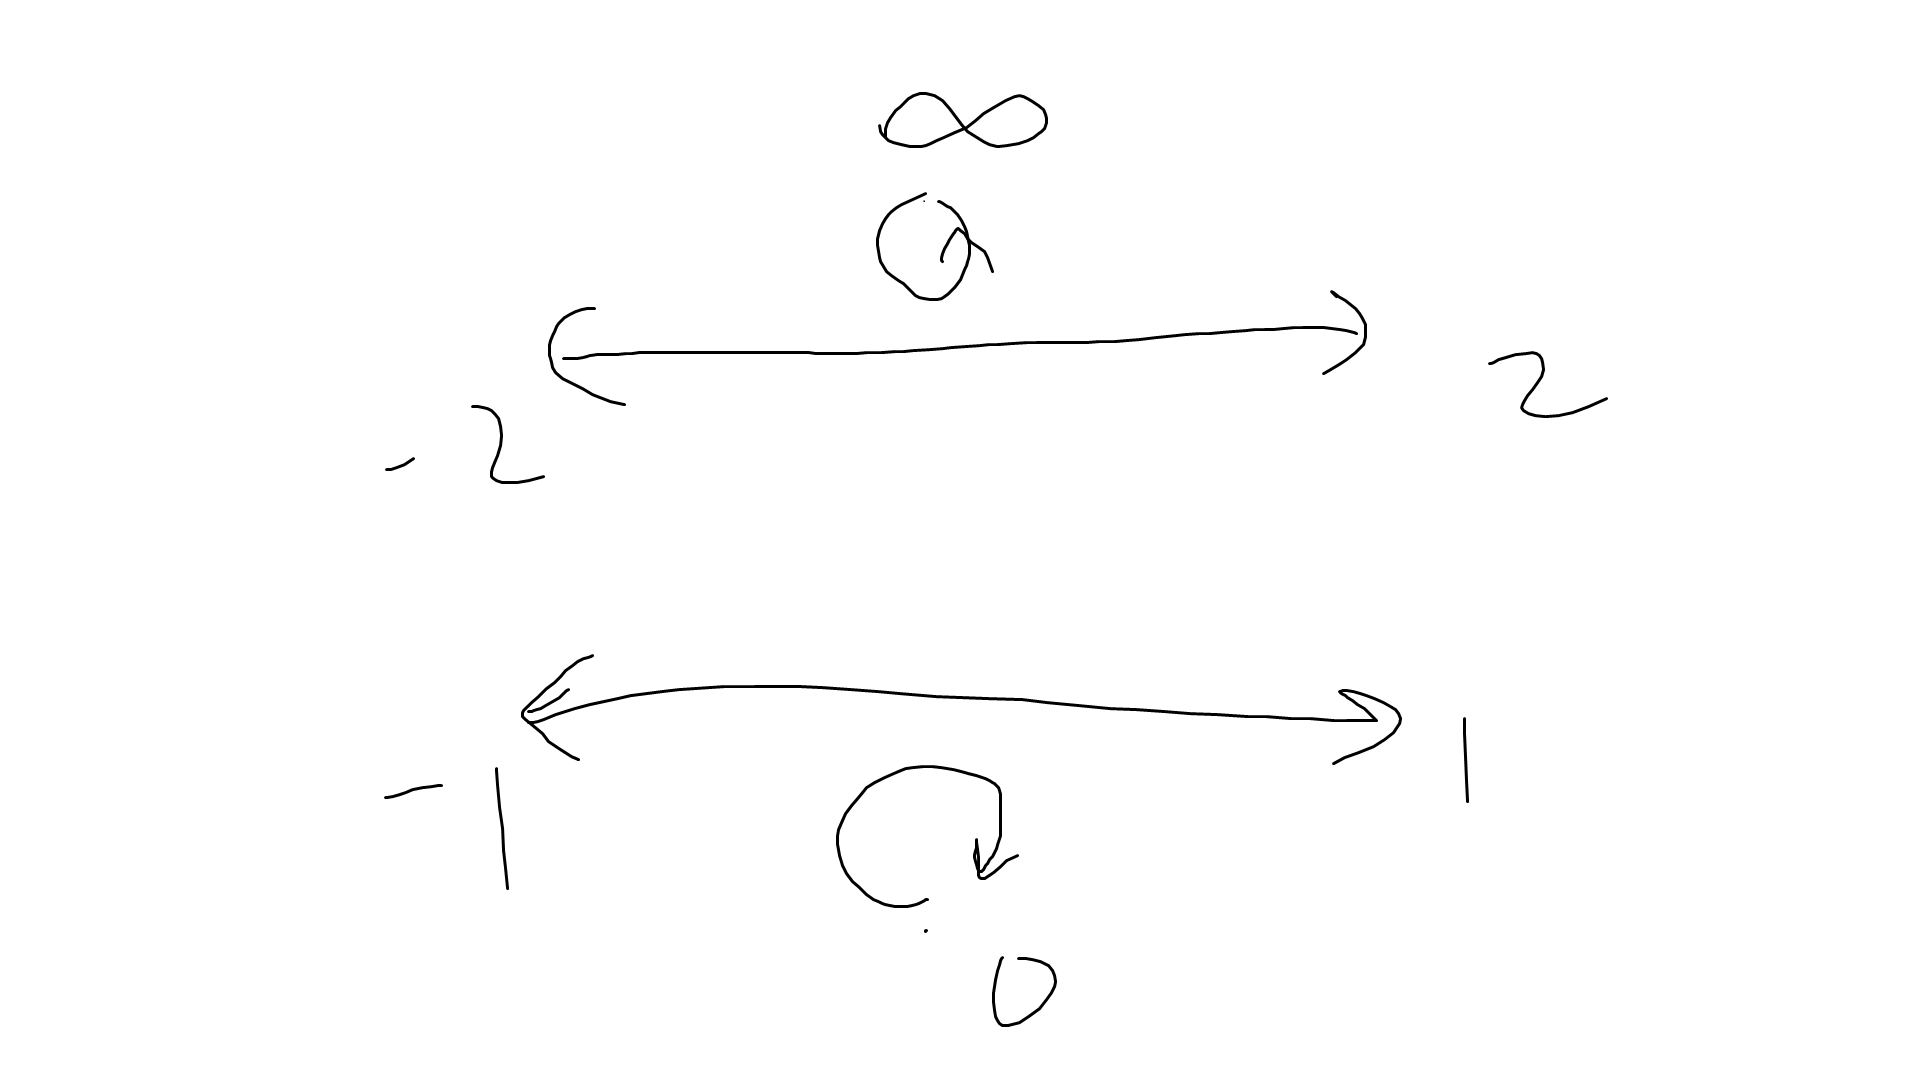
\includegraphics[scale=0.4]{GRM_01}

so is an even permutation. Then
\begin{equation*}
\begin{aligned}
\left[\begin{matrix}
0 & 1\\
-1 & 0
\end{matrix}\right]
\end{aligned}
\end{equation*} 
sends

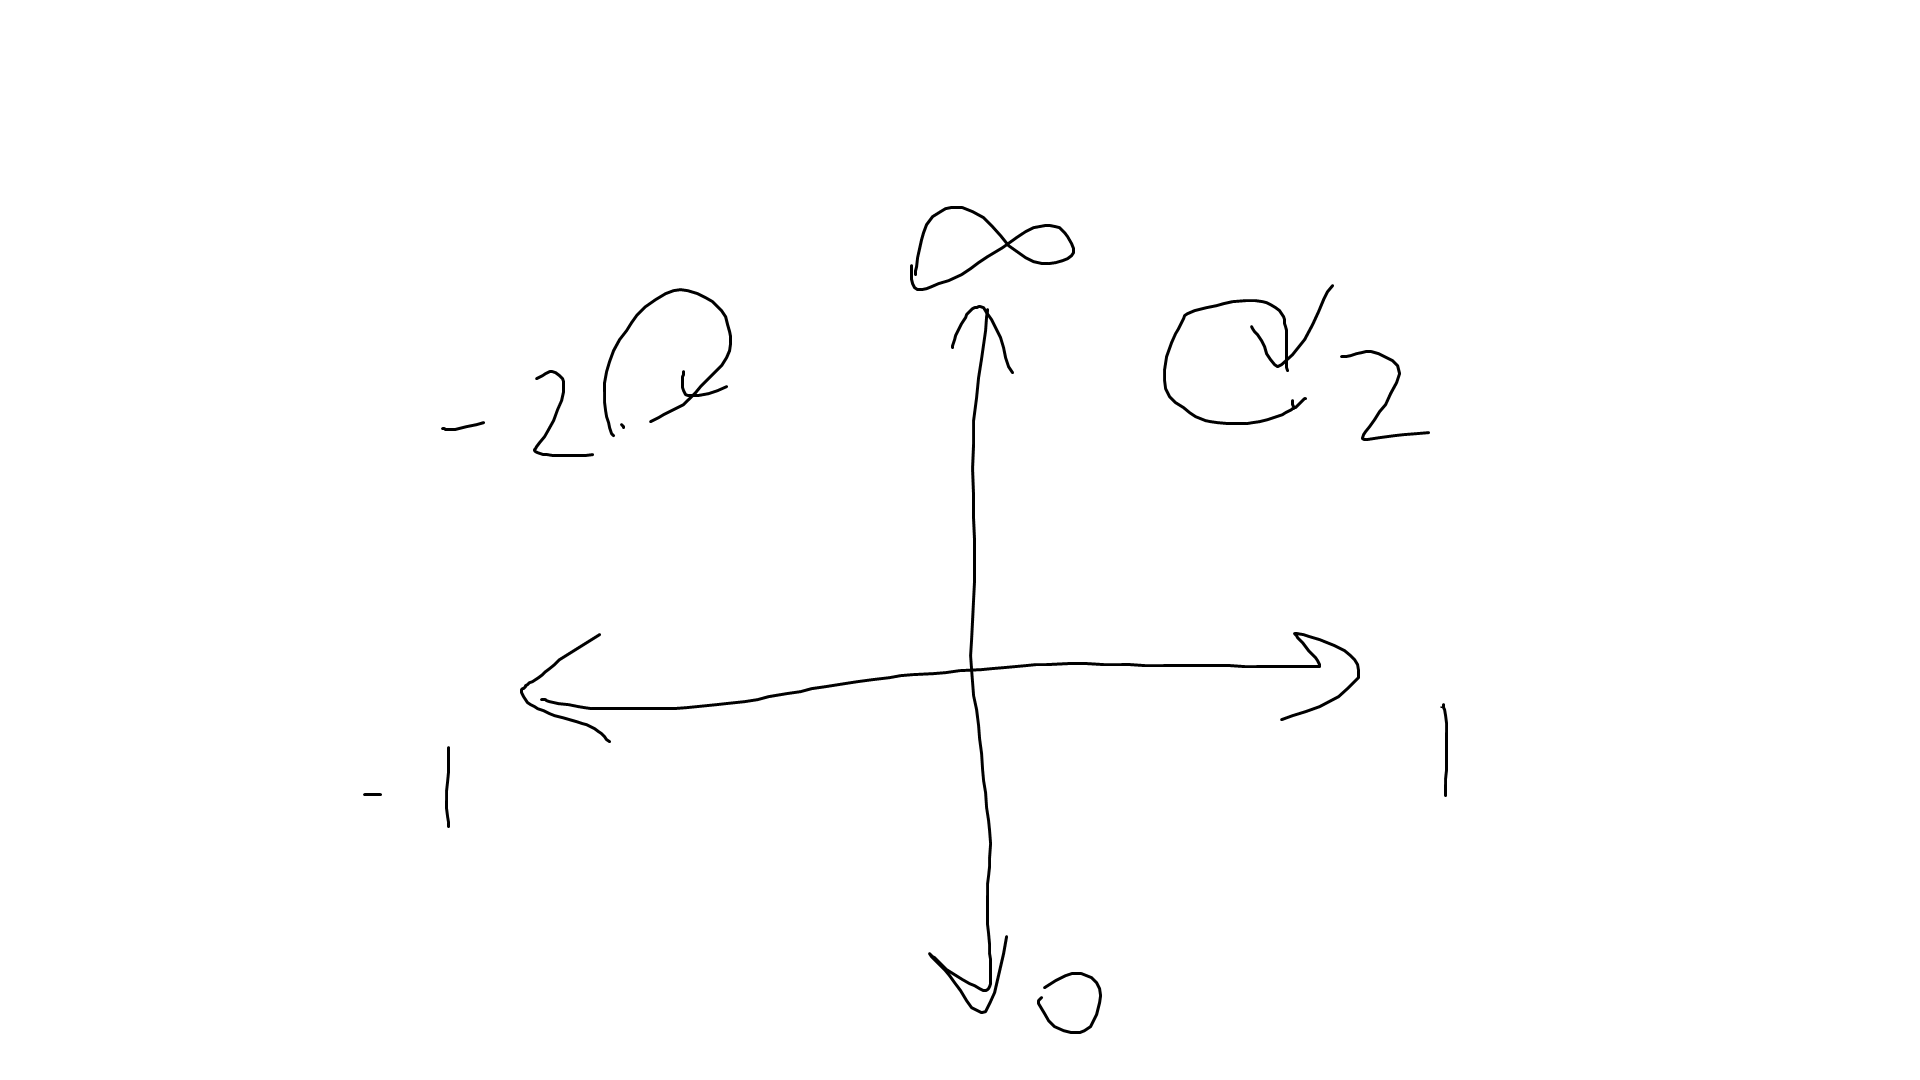
\includegraphics[scale=0.4]{GRM_02}

is also even. So they are both in $A_6$.

\end{proof}
\end{eg}

\newpage

\section{Rings}

In this course we only consider commutative rings with a multiplicative identity. Many of the things we are going to prove in this course will not hold without these two properties.

\subsection{Definitions}
\begin{defi}
A \emph{ring} is a quintuple $(R,+,\cdot,0_R,1_R)$ s.t. \\
(R1) $(R,+,0_R)$ is an abelian group;\\
(R2) The operation $- \cdot -$: $R \times R \to R$ is associative, and satisfies $1_R \cdot r = r = r \cdot 1_R$.\\
(R3) $r \cdot (r_1+r_2) = r \cdot r_1 + r \cdot r_2$, and $(r_1+r_2) \cdot r = r_1 \cdot r + r_2 \cdot r$ (Distributivity).

A ring is \emph{commutative} if in addition $a \cdot b = b \cdot a$ $\forall a,b \in R$.

From now on every ring we discuss will by default be commutative and has a multiplicative identity.
\end{defi}

\begin{defi}
If $(R,+,\cdot,0_R,1_R)$ is a ring ans $S \subset R$ is a subset, then it is called a \emph{subring} if $0_R,1_R \in S$ and $+,\cdot$ make $S$ into a ring in its own right.
\end{defi}

\begin{eg}
We have $\Z \leq \Q \leq \R \leq \C$ as rings with the usual $0,1,+,\cdot$.
\end{eg}

\begin{eg}
$\Z[i] = \{a+ib\in \C \mid a,b \in \Z\} \leq \C$ is the subring called \emph{Gaussian integers}. 
\end{eg}

\begin{eg}
$\Q[\sqrt{2}] = \{ a+\sqrt{2} \cdot b \in \R \mid a,b \in \Q \} \leq \R$ is a subring.
\end{eg}

\begin{defi}
An element $r \in R$ is a \emph{unit} if there is a $s \in R$ s.t. $sr = 1_R$.

Note that this depends not only on the element but only on which ring we are talking about: $2 \in \Z$ is not a unit, but $2 \in \Q$ is.

If every $r \in R$ with $r \neq 0_R$ is a unit, then $R$ is called a field.
\end{defi}

\begin{notation}
If $x \in R$, write $-x \in R$ for the inverse of $x$ in $(R,+,0_R)$. We will write $y-x = y+(-x)$.
\end{notation}

\begin{eg}
$0_R+0_R = 0_R$, so $r \cdot (0_R+0_R) = r\cdot 0_R$, i.e. $r\cdot 0_R + r\cdot 0_R = r\cdot 0_R$, so $r\cdot 0_R = 0_R$. So if $R \neq \{0\}$, then $0_R \neq 1_R$, and $0_R$ is never a unit.

However, $(\{0\},+,\cdot,0,0)$ \emph{is} a valid ring.
\end{eg}

\begin{eg}
If $R,S$ are rings, then $R \times S$ has the state of a ring via componentwise addition and multiplication, with $1=(1_R,1_S)$, $0 =(0_R,0_S$.

Note that in this ring, $e_1 = (1_R,0_S)$, $e_2 = (0_R,1_S$, then $e_1^2 =e_1$ and $e_2^2 = e_2$, and $e_1+e_2 = 1$.
\end{eg}

\begin{eg}
Let $R$ be a ring. A \emph{polynomial} $f$ over $R$ is an expression
\begin{equation*}
\begin{aligned}
f=a_0+a_1X+a_2X^2 + ... + a_n X^n
\end{aligned}
\end{equation*}
with $a_i \in R$. $X^i$ is just a symbol.

We will consider $f$ and 
\begin{equation*}
\begin{aligned}
a_0+a_1 X +... + a_n X^n + 0_R \cdot X^{n+1}
\end{aligned}
\end{equation*}
as equal. The \emph{degree} of $f$ is the largest $n$ s.t. $a_n \neq 0$.

If in addition, $a_n = 1_R$, then we say $f$ is \emph{monic}.

We write $R[X]$ for the set of all polynomials over $R$.

If $g=b_0+...+b_m X^m$, then we define addition and multiplication by the usual way:
\begin{equation*}
\begin{aligned}
f+g &= \sum_{i=0} (a_i+b_i) X^i\\
f\cdot g &= \sum_i \left(\sum_0^i a_jb_{i-j}\right)X^i
\end{aligned}
\end{equation*}

Now consider $R$ as a subring of $R[X]$, given by the polynomials of degree $0$. In particular, $1_R \in R$ gives the multiplicative identity element of $R[X]$.
\end{eg}

\begin{eg}
Write $R[[x]]$ for the ring of \emph{formal power series}, i.e.
\begin{equation*}
\begin{aligned}
f =a_0+a_1 X + a_2 X^2 + ...
\end{aligned}
\end{equation*}
with the same addition and multiplication.

Consider $\Z/2[X]$ and an element $f = X+X^2$. Then
\begin{equation*}
\begin{aligned}
f(0)=0+0=0,
f(1) = 1+1=0
\end{aligned}
\end{equation*}
But definitely $f \neq 0$. So we see the reason why we don't think $f$ as functions despite that they do give functions. They are just elements in a particular ring.
\end{eg}

\begin{eg}
The \emph{Laurent polynomials} $R[X,X^{-1}]$ is the set of 
\begin{equation*}
\begin{aligned}
f=\sum_{i \in \Z} a_i X^i
\end{aligned}
\end{equation*}
s.t. only finitely many $a_i$ are non-zero.
\end{eg}

\begin{eg}
The ring of \emph{Laurent series} are those expressions
\begin{equation*}
\begin{aligned}
f = \sum_{i\in \Z} a_i X_i
\end{aligned}
\end{equation*}
with only finitely many $i<0$ s.t. $a_i \neq 0$ (i.e. formal power series in the positive part and polynomial in the negative part). This is to make the sum in each coefficient a finite sum, as we didn't even define infinite sums in rings.
\end{eg}

\begin{eg}
If $R$ is a ring and $X$ is a set, the set $R^X$ of all functions $f: X \to \R$ is a ring, with operations
\begin{equation*}
\begin{aligned}
(f+g) (X) &= f(X) + g(X),\\
(fg) (X) &= f(X) \cdot g(X).
\end{aligned}
\end{equation*}
The multiplicative identity element is the function $1(X) = 1_R$ for all $X$, and the same for the zero element.

Observe $\R^\R \supsetneq$ set of continuous $f:\R \to \R$ $\supset$ polynomials $\R \to \R$ = $\R[X]$. So $\R[X] \subsetneq \R^\R$.
\end{eg}

\subsection{Homomorphisms, ideals, quotients, and isomorphisms}
\begin{defi}
A function $\phi: R \to S$ between rings is a \emph{homomorphism} if\\
(H1) $\phi(r_1+r_2) = \phi(r_1)+\phi(r_2)$, i.e. $\phi$ is a group homomorphism between the additive groups of $R$ and $S$;\\
(H2) $\phi(r_1r_2) \phi(r_1) \phi(r_2)$;\\
(H3) $\phi(1_R) = 1_S$.

If in addition, $\phi$ is a bijection, then we say it is an \emph{isomorphism}.

The \emph{kernel} of $\phi:R \to S$ is
\begin{equation*}
\begin{aligned}
\ker(\phi) = \{r \in R | \phi(r) = 0\}
\end{aligned}
\end{equation*}
\end{defi}

\begin{lemma}
$\phi:R \to S$ is injective if and only if $\ker(\phi) = \{0\}$.
\begin{proof}
Note that $\phi:(R,+,0_R) \to (S,+,0_S)$ is a group homomorphism, and its kernel as a group homomorphism is also $\ker(\phi)$. So by theorems in groups we get the desired result.
\end{proof}
\end{lemma}

\begin{defi}
A subset $I \subset R$ is an \emph{ideal}, written $I \triangleleft R$, if\\
(I1) $I$ is a subgroup of $(R,+)$;\\
(I2) If $x \in I$, $r \in R$, then $x \cdot r \in I$ (strong multiplicative closure).

We say $I \triangleleft R$ is proper if $I \neq R$.
\end{defi}

\begin{lemma}
If $\phi:R \to S$ is a homomorphism, then $\ker(\phi) \triangleleft R$.
\begin{proof}
(I1) holds for $\ker(\phi)$ since $\phi$ is a group homomorphism. 

Now let $x \in \ker(\phi)$, $r \in R$. Then
\begin{equation*}
\begin{aligned}
\phi(r \cdot x) = \phi(r) \cdot \phi(x) = \phi(r) \cdot 0_S = 0_S
\end{aligned}
\end{equation*}
So $r \cdot x \in \ker(\phi)$.
\end{proof}
\end{lemma}

\begin{eg}
If $I \triangleleft R$ and $1_R \in I$, then for any $r \in R$, we have
\begin{equation*}
\begin{aligned}
r = r \cdot 1 \in I,
\end{aligned}
\end{equation*}
so $I=R$. In short, proper ideals never include $1$, so are never subrings.
\end{eg}

\begin{eg}
If $R$ is a field, then $\{0\}$ and $R$ are the only ideals. This is reversible: If $\{0\}$ and $R$ are the only ideals, then $R$ is a field.
\end{eg}

\begin{eg}
In the ring $\Z$, all ideals are of the form $n\Z$ for some $n \in \Z$, where
\begin{equation*}
\begin{aligned}
n\Z =\{...,-2n,-n,0,n,2n,...\}
\end{aligned}
\end{equation*}
\begin{proof}
$n \Z$ is certainly an ideal. Let $I \triangleleft \Z$ be an ideal. Let $n \in I$ be the smallest positive element. Then $n \Z \subset I$. If this is not an equality, choose $m \in I\backslash n\Z$. Then $m=n \cdot q + r$ for some $0\leq r \leq n-1$. If $r=0$ then $m \in I$, a contradiction. So
\begin{equation*}
\begin{aligned}
r=m-n\cdot q < n
\end{aligned}
\end{equation*}
is in the ideal $I$. Contradiction.
\end{proof}
\end{eg}

\begin{defi}
For an element $a \in R$, write
\begin{equation*}
\begin{aligned}
(a) = \left\{a \cdot r | r \in R\right\}
\end{aligned}
\end{equation*}
the \emph{ideal generated by $a$}. More generally, for a list $a_1,...,a_s$, write
\begin{equation*}
\begin{aligned}
(a_1,...,a_s) = \left\{\sum_i a_i r_i | r_i \in R\right\}
\end{aligned}
\end{equation*}
which somewhat resembles the linear combinations in a vector space.

Even more generally, if $A \subseteq R$ is a subset, then the ideal generated by $A$ is
\begin{equation*}
\begin{aligned}
\left(A\right) = \left\{\sum_{a \in A} a \cdot r_a | r_a \in R, \text{only finitely many }r_a \neq 0\right\}.
\end{aligned}
\end{equation*}
since we have no definition of infinite sums in rings.

If an ideal $I\triangleleft R$ is of the form $(a)$, then we say that $I$ is a \emph{principal ideal}.
\end{defi}

\begin{eg}
In $\Z$ we have
\begin{equation*}
\begin{aligned}
n\Z = (n) \triangleleft \Z
\end{aligned}
\end{equation*}
is principal.
\end{eg}

\begin{eg}
In $\C[X]$, the polynomials with constant coefficient $0$ forms an ideal, which is just $(X)$ (check). This is also principal.
\end{eg}

\begin{prop}
Let $I \triangleleft R$ be an ideal. Define the \emph{quotient ring} $R/I$ to be the set of cosets $r+I$ (i.e. $(R,+,0)/$normal subgroup $I$), with addition and multiplication given by\\
$\bullet$ $(r_1+I)+(r_2+I) = r_1+r_2+I$,\\
$\bullet$ $(r_1+I)+(r_2+I) = r_1r_2 + I$,\\
and $0_{R/I} =0_R+I$, $1_{R/I} = 1_R+I$. 

This is a ring, and the quotient map $R \to R/I$ by $r \to r+I$ is a ring homomorphism.
\begin{proof}
We already know that $(R/I,+,0)$ is an abelian group. And addition as described above is well-defined. If $r_1+I=r'_1+I$, $r_2+I = r'_2+I$, then $r'_1-r_1 =a_1 \in I$, $r'_2-r_2 = a_2 \in I$. So
\begin{equation*}
\begin{aligned}
r'_1r'_2 = (r_1+a_1)(r_2+a_2)=r_1r_2+r_1a_2+a_1r_2+a_1a_2 = r_1r_2 + a
\end{aligned}
\end{equation*}
for some $a \in I$, i.e. $r'_1r'_2 + I = r_1 r_2 + I$. So multiplication is well-defined. The ring axioms for $R/I$ then follow from those of $R$.
\end{proof}
\end{prop}

\begin{eg}
$n\Z \triangleleft \Z$, so have a ring $\Z/n\Z$. This has elements $0+n\Z,1+n\Z,2+n\Z,...,(n-1)+n\Z$, and addition and multiplication are modular arithmetic $\pmod n$.
\end{eg}

\begin{eg}
$(X) \triangleleft \C[X]$, so we have a ring $\C[X] / (X)$. Then
\begin{equation*}
\begin{aligned}
a_0+a_1X+a_2X^2+...+a_nX^n + (X) = a_0 + (X).
\end{aligned}
\end{equation*}
If $a_0+(X) = b_0+(X)$, then $a_0-b_0 \in (X)$. So $X | a_0-b_0$, i.e. $a_0=b_0$.

So consider
\begin{equation*}
\begin{aligned}
\phi: \C[X] / (X) &\longleftarrow &\C\\
a+(X) & \longleftarrow & a
\end{aligned}
\end{equation*}
is surjective and injective. So $\phi$ is a bijection.

Observe that $\phi$ is a ring homomorphism. The inverse is $f+(X) \to f(0)$.
\end{eg}

\begin{prop} (Euclidean algorithm for polynomials)\\
Let $F$ be a field and $f,g \in F[X]$, then we may write
\begin{equation*}
\begin{aligned}
f = g\cdot q + r
\end{aligned}
\end{equation*}
with $\deg(r) < \deg(g)$.
\begin{proof}
Let\\
$\deg(f) = n$, so $f=a_0+a_1X + ... + a_nX^n$ with $a_n \neq 0$;\\
$\deg(g) = m$, so $g=b_0+b_1X + ... + b_mX^m$ with $b_m \neq 0$.

If $n<m$, let $q=0$ and $r=f$.

Suppose $n \geq m$, and proceed by induction on $n$, Let
\begin{equation*}
\begin{aligned}
f_1 = f-g \cdot X^{n-m} \cdot a_n b_m^{-1}
\end{aligned}
\end{equation*}
we can do this because $F$ is a field, so $b_m$ has an inverse.

This has degree smaller than $n$.

If $n=m$, then $f = gX^{n-m}a_nb_m^{-1} + f_1$ where $\deg(f_1)<n=m$.

If $n>m$, by induction on degree, we have $f_1 = g\cdot q_1 + r$ with $\deg(r) < \deg(g)$. So $f=gX^{n-m}a_n+b_m^{-1} + g\cdot q_1+r = g (X^{n-m}b_m^{-1} + q_1) +r$ as required.
\end{proof}
\end{prop}

\begin{eg}
Consider $(X^2+1) \triangleleft \R[X]$, and $R=\R[X]/(X^2+1)$. Elements of $R$ are of the form $f+(X^2+1)$. By Euclidean algorithm we have $f=q\cdot (X^2+1) + r$ with $\deg(r) < 2$. So $f+(X^2+1) = r + (X^2+1)$. So every coset is represented by a polynomial $r$ of degree at most $1$.

If $a_1+b_1X + (X^2+1) = a_2+b_2X + (X^2+1)$, then
\begin{equation*}
\begin{aligned}
X^2+1 | (a_1+b_1X)-(a_2+b_2X)
\end{aligned}
\end{equation*}
But by degree we know that $(a_1+b_1X) - (a_2+b_2X) = 0$. So take
\begin{equation*}
\begin{aligned}
\phi:\R[x]/(X^2+1) &\to \C\\
a+bX+(X^2+1) &\to a+bi
\end{aligned}
\end{equation*}
This is a bijection. It sends addition to addition, and multiplication satisfies
\begin{equation*}
\begin{aligned}
&\phi((a+bX+(X^2+1)) \cdot (c+dX+(X^2+1)))\\
&=\phi(ac+(bc+ad)X + bdX^2 + (X^2+1))\\
&=\phi(ac+(bc+ad)X + bd(-1) + bd(X^2+1) + (X^2+1))\\
&=\phi((ac-bd) + (bc+ad)X + (X^2+1))\\
&=(ac-bd)+(bc+ad)i\\
&=(a+ib)(c+id)
\end{aligned}
\end{equation*}
So $\phi$ is a homomorphism. So $\R[x] / (X^2+1) \cong \C$.
\end{eg}

We also have $\Q[x]/(X^2-2) = \Q[\sqrt{2}] \subseteq \R$.

\begin{thm} (First isomorphism theorem)\\
Let $\phi:R \to S$ be a ring homomorphism. Then $\ker(\phi) \triangleleft R$, $\im(\phi) \leq S$, and $R/\ker(\phi) \cong \im(\phi)$ by $r+\ker(\phi) \to \phi(r)$.
\end{thm}

\begin{thm} (Second isomorphism theorem)\\
Let $R \subset S$, $J \triangleleft S$. Then $R\cap J \triangleleft R$, $(R+J)/J = \{r+J | r \in R\} \leq S/J$, and $R / R\cap J = (R+J)/J$.
\end{thm}

\begin{thm} (Subring correspondence)\\
We have a bijection between subrings of $R/I$ and subrings of $R$ containing $I$ by:\\
$S/I \leq R/I \leftarrow I \triangleleft S \leq R$\\
$L \leq R/I \rightarrow \{r\in R | r+I \in L\}$, and the same map gievs a bijection between ideals of $R/I$ and ideals of $R$ containing $I$ by
\begin{equation*}
\begin{aligned}
\end{aligned}
J/I \triangleleft R/I \leftrightarrow I \triangleleft J \triangleleft R.
\end{equation*}
\end{thm}

\begin{thm} (Third isomorphism theorem)\\
Let $I,J \triangleleft R$, $I \subset J$. Then $J/I \triangleleft R/I$ and $(R/I)/(J/I) \cong R/J$.
\end{thm}

\begin{eg}
Consider the homomorphism $\phi: \R[X] \to \C$ by substituting in $X=i$, which is onto. We know
\begin{equation*}
\begin{aligned}
\ker(\phi) = \{f \in \R[x] | f(i) = 0\} = (X^2+1)
\end{aligned}
\end{equation*}
because real polynomials with $i$ as a root also have $-i$ as a root. So are divisible by $(X-i)(X+i) = (X^2+1)$. Then by first isomorphism theorem,
\begin{equation*}
\begin{aligned}
\R[X] / (X^2+1) \cong \C
\end{aligned}
\end{equation*}
(Compare with the previous proof).
\end{eg}

\begin{defi}
For any ring $R$, there is a unique homomorphism
\begin{equation*}
\begin{aligned}
\iota:\Z &\to \R\\
1 &\to 1_R\\
n>0 &\to 1_R+1_R+...+1_R \ (n \text{ times})\\
n<0 &\to -(1_R+1_R+...+1_R)\ (-n \text{ times})\\
\end{aligned}
\end{equation*}
Note that $\ker(\iota) \triangleleft \Z$, so $\ker(i) = n\Z$ for some $n \geq 0$. This $n \geq 0$ is called the \emph{characteristic} of the ring $R$.
\end{defi}

\begin{eg}
$\Z \leq \Q \leq \R \leq \C$ all have characteristic $0$, while $\Z/n$ has characteristic $n$.
\end{eg}

\subsection{Integral domains, field of fractions, maximal and prime ideal}
One thing to remember:
\begin{equation*}
\begin{aligned}
Field \implies ED \implies PID \implies UFD \implies ID.
\end{aligned}
\end{equation*}

The interesting bits start here.

\begin{defi}
A non-zero ring $R$ is called an \emph{integral domain (ID)} if for all $a,b \in R$, $a \cdot b = 0 \implies a=0$ or $b=0$.

We call $x$ a \emph{zero divisor} in $R$ if $x\neq 0$ but $\exists y \neq 0$ s.t. $xy = 0$.
\end{defi}

\begin{eg}
All fields are integral domains. If $xy=0$ with $y \neq 0$, then $xyy^{-1} = 0$ i.e. $x=0$.

A subring of an integral domain is an integral domain, so $\Z \leq \Q$ and $\Z[i] \leq \C$ are integral domains.
\end{eg}

\begin{defi}
A ring $R$ is a \emph{principal ideal domain (PID)} if it is an integral domain and every ideal is principal.
\end{defi}

For example, $\Z$ is a principal ideal domain.

\begin{lemma}
A finite integral domain is a field.
\begin{proof}
Let $a \neq 0 \in R$, and consider
\begin{equation*}
\begin{aligned}
a \cdot -: R &\to R\\
b &\to ab
\end{aligned}
\end{equation*}
This is a homomorphism of abelian groups and its kernel is $\{b \in R | ab=0\} = \{0\}$. So $a\cdot -$ is injective. But $R$ is finite. So $a \cdot -$ is bijective. In particular, $\exists b \in R$ s.t. $ab=1$. So $R$ is a field.
\end{proof}
\end{lemma}

\begin{lemma}
Let $R$ be an integral domain, then $R[X]$ is also an integral domain.
\begin{proof}
Let $f=\sum_{i=0}^n a_i X^i$ and $a_n \neq 0$, $g=\sum_{i=0}^m b_i X^i$ and $b_m \neq 0$ be non-zero polynomials. Then the largest power of $X$ in $fg$ is $X^{n+m}$ and its coefficient is $a_nb_m \neq 0$ as $R$ is an ID. So $fg \neq 0$.
\end{proof}
\end{lemma}

Iterating this, we have
\begin{equation*}
\begin{aligned}
R[X_1,...,X_n] = (((R[X_1])[X_2])...[X_n])
\end{aligned}
\end{equation*}
is an integral domain.

\begin{thm}
Let $R$ be an ID. There is a \emph{field of fractions} $F$ of $R$ with the following properties:\\
(i) $F$ is a field;\\
(ii) $R \leq F$;\\
(iii) every element of $F$ is of the form $a \cdot b^{-1}$ for $a,b \leq R \leq F$.
\end{thm}
\begin{proof}
Consider
\begin{equation*}
\begin{aligned}
S=\{(a,b)\in R\times R| b\neq 0\}
\end{aligned}
\end{equation*}
with the equivalence relation $(a,b) \sim (c,d) \iff ad=bc \in R$. This is reflexive and symmetric. For transitivity, if 
\begin{equation*}
\begin{aligned}
(c,d) \sim (e,f)
\end{aligned}
\end{equation*}
Then $(ad)f = (bc)f = b(cf) = b(ed) \implies d(af-be) =0 $. But $d \neq 0$. So $af-be = 0$.

Let $F = S/\sim$. Write $[(a,b)] = \frac{a}{b}$ and define
\begin{equation*}
\begin{aligned}
\frac{a}{b} + \frac{c}{d} = \frac{ad+bc}{bd},\\
\frac{a}{b} \cdot \frac{c}{d} = \frac{ab}{cd}.
\end{aligned}
\end{equation*}
and $0=\frac{0}{1}$, $1=\frac{1}{1}$.

If $\frac{a}{b} \neq 0$ then $a \cdot 1 \neq 0 \cdot b$, i.e. $a \neq 0$. Then $\frac{b}{a} \in F$, so $\frac{a}{b} \cdot \frac{b}{a} = \frac{1}{1}$. So $\frac{a}{b}$ has an inverse, so $F$ is a field.

We make $R \leq F$ by $\phi:R \to F$ by $r \to \frac{r}{1}$.
\end{proof}

\begin{eg}
The field of fractions of $\Z$ is $\Q$, and that of $\C[z]$ is the rational polynomial fractions in $z$.
\end{eg}

Note: the ring $\{0\}$ is \emph{not} afield.

\begin{lemma}
A (non-zero) ring is a field iff its only ideals are $\{0\}$ and $R$.
\begin{proof}
If $I \triangleleft R$ is a non-zero ideal, then it contains $a \neq 0$. But an ideal containing a unit must be the whole ring. On the other hand, let $x \neq 0 \in R$, Then $(x)$ must be $R$, as it is \emph{not} the zero ideal. So $\exists y \in R$ s.t. $xy = 1_R$. So $X$ is a unit.
\end{proof}
\end{lemma}

\begin{defi}
An ideal $I \triangleleft R$ is \emph{maximal} if there is no proper ideal which properly contains $I$.
\end{defi}

\begin{lemma}
An ideal $I$ is maximal iff $R/I$ is a field.
\begin{proof}
$R/I$ is a field $\iff$ $I/I$ and $R/I$ are the only ideals in $R/I$ $\iff$ $I,R\ triangleleft$ are the only ideals containing $I$ by ideal correspondence.
\end{proof}
\end{lemma}

\begin{defi}
An ideal $I \triangleleft R$ is \emph{prime} if $I$ is proper, and if $a,b \in R$ are s.t. $a \cdot b \in I$, then $a\in I$ or $b \in I$.
\end{defi}

\begin{eg}
The ideal $n\Z \triangleleft \Z$ is prime if and only if $n$ is zero and a prime number: if $p$ is prime and $a \cdot b \in p\Z$, then $p | a \cdot b$, so $p|a$ or $p|b$, i.e. $a \in p\Z$ or $b \in p\Z$.

Conversely, if $n=uv$ is composite, $u\cdot v \in n\Z$ but $u,v \not\in n\Z$.
\end{eg}

\begin{lemma}
$I \triangleleft R$ is prime iff $R/I$ is an integral domain.\\
Note that this shows that every maximal ideal is prime since fields are integral domains.
\end{lemma}
\begin{proof}
Suppose $I$ is prime. Let $a+I,b+I \in R/I$ be s.t. $(a+I)(b+I) = 0$, i.e. $ab+I=0$, so $ab \in I$. But $I$ is prime, so $a \in I$ or $b \in I$. So $a+I = 0+I$ or $b+I = 0+I$ is the zero element in $R/I$. So $R/I$ is an integral domain.

For the other direction, suppose $R/I$ is an integral domain. Let $ab \in I$. Then $ab+I = 0$, so $(a+I)(b+I)=0$. So $a+I = 0+I$ or $b+I = 0+I$, i.e. $a \in I$ or $b \in I$.
\end{proof}

\begin{lemma}
If $R$ is an integral domain, then its characteristic is $0$ or a prime number.
\begin{proof}
Let $\iota:\Z \to R$ with $1 \to 1_R$. Consider $\ker(\iota) = n\Z$. By 1st isomorphism theorem, $\Z / n\Z \cong \im(\phi) \leq R$ as a subring of an integral domain is again an integral domain, $Z/n\Z$ is an integral domain, so $n\Z \triangleleft \Z$ is prime. So $n$ is zero or a prime number.
\end{proof}
\end{lemma}

\subsection{Factorisation in integral domains}
Suppose throughout this section that $R$ is an integral domain.\\
\begin{defi}
1) An element $a\in R$ is a unit if there is $b\in R$ s.t. $ab=1$. Equivalently, $\left(a\right)=R$.\\
2) $a$ divides $b$ if there is $c\in R$ s.t. $b=a\cdot c$. Equivalently, $\left(b\right) \subset \left(a\right)$.\\
3) $a,b\in R$ are associates if $a=b\cdot c$ with $c$ a unit. Equivalently, $\left(a\right)=\left(b\right)$, or $a|b$ and $b|a$.\\
4) $a\in R$ is irreducible if it is not 0, not a unit, and if $a=x\cdot y$ then $x$ or $y$ is a unit.\\
5) $a\in R$ is prime if it is not 0, not a unit, and when $a|x\cdot y$ then $a|x$ or $a|y$.\\

Note that $2\in \Z$ is prime, but $2\in \Q$ is not.\\
$2x\in \Q[x]$ is irreducible, $2x\in \Z[x]$ is not irreducible.
\end{defi}

\begin{lemma}
$\left(a\right)$ is a prime ideal in $R \iff r=0$ or $r$ is prime in $R$.
\begin{proof}
1) let $\left(r\right)$ be a prime, $r\neq 0$. As $\left(r\right) \neq R$, $r$ is not a unit.\\
Suppose $r|a\cdot b$. Then $a\cdot b\in \left(r\right)$, but $\left(r\right)$ is prime. So $a\in\left(r\right)$ or $b\in\left(r\right)$. So $r|a$ or $r|b$. So $r$ is prime in $R$.\\
2) if $r=0$ then $(0)$ is a prime ideal since $R$ is an integral domain.\\
Now let $r\neq 0$ and be prime in $R$.\\
Let $ab\in\left(r\right)$. Then $r|ab$. So $r|a$ or $r|b$. So $a\in\left(r\right)$ or $b\in\left(r\right)$. So $\left(r\right)$ is a prime ideal in $R$.
\end{proof}
\end{lemma}

\begin{lemma}
if $r\in R$ is prime, then it is irreducible.
\begin{proof}
let $r\in R$ be prime, and suppose $r=a\cdot b$.\\
As $r$ is prime, $r|a$ or $r|b$.\\
Suppose $r|a$. So $a=r\cdot c$. Then $r=r\cdot c\cdot b$.\\
As $R$ is an integral domain, \\
$r\left(c\cdot b-1\right)=0 \implies c\cdot b=1$.\\
So $b$ is a unit. So $r$ is irreducible.
\end{proof}
\end{lemma}

\begin{eg}
Let $R=\Z[\sqrt{-5}]=\left\{a+b\sqrt{-5}|a\cdot b\in\Z\right\}\subseteq \C$.\\
$\C$ is a field and $R$ is a subring, so $R$ is an integral domain.\\
Consider the "norm":\\
\begin{equation*}
\begin{aligned}
N:R &\to \Z \geq 0\\
a+b\sqrt{-5} &\to a^2+5b^2\\
z &\to z\overline{z}=|z|^2.
\end{aligned}
\end{equation*}
This satisfies $N\left(zw\right)=N\left(z\right)\cdot N\left(w\right)$.\\
If $r\cdot s=1$ then $1=N\left(1\right)=N\left(r\cdot s\right)=N\left(r\right)\cdot N\left(s\right)$.\\
So $N\left(s\right)=N\left(r\right)=1$. So any unit has normal 1.\\
i.e. $a^2+5b^2=1$. Then $a=\pm 1, b=0$: only $\pm 1\in R$ are units.\\
\textbf{Claim}: $2\in R$ is irreducible:\\
Suppose $2=ab$. Then $4=N\left(a\right) N\left(b\right)$.\\
Note that nothing in $R$ has norm 2. So WLOG $N\left(a\right)=1,N\left(b\right)=4$. So $a$ is a unit. So 2 is irreducible.\\
Similarly $3,1+\sqrt{-5},1-\sqrt{-5}$ are irreducible (no $r$ with $N\left(r\right)=3$).\\
Note that $\left(1+\sqrt{-5}\right)\left(1-\sqrt{-5}\right)=6=2\cdot 3$.\\
\textbf{Claim}: 2 does not divide $1 \pm \sqrt{-5} \implies 2$ is not prime:\\
if $2|1+\sqrt{-5}$, then $N\left(2\right)|N\left(1+\sqrt{-5}\right)$, i.e. $4|6$, contradiction.\\
\textbf{Lessons}: 1) irreducible doesn't imply prime in general.\\
2) $\left(1+\sqrt{-5}\right)\left(1-\sqrt{-5}\right) = 2\cdot 3$. So factorisation into irreducibles might not be unique.
\end{eg}

\begin{defi}
an integral domain $R$ is a \emph{Euclidean domain}(ED) if there is a function $\varphi: R \backslash \left\{0\right\}\to \Z\geq 0$, a "Euclidean function", such that:\\
1) $\varphi \left(a\cdot b\right) \geq \varphi\left(b\right)$ for all $a,b\neq 0$;\\
2) if $a,b\in R$ with $b\neq 0$, there are $q,r\in R$ s.t. $a=b\cdot q+r$, such that $r=0$ or $\varphi\left(r\right)<\varphi\left(b\right)$ ($r$ is "strictly smaller than" $b$).
\end{defi}

\begin{eg}
1) $\Z$ is a Euclidean domain with $\varphi\left(n\right)=|n|$.\\
2) $F[x]$ with $F$ a field is a Euclidean domain with $\varphi\left(f\right)=\deg\left(f\right)$.\\
3) $\Z[i]=R$ is Euclidean domain, with $\varphi\left(z\right)=N\left(z\right)=|z|^2=z\overline{z}$:\\
	i) $\varphi\left(zw\right)=\varphi\left(z\right)\varphi\left(w\right) \geq \varphi\left(z\right)$, as $\varphi\left(w\right)\in \Z^+$ for $w\neq 0$;\\
	ii) let $a,b\in\Z[i]$. Consider $\frac{a}{b}\in\C$.\\
		We know that $\exists q\in\Z[i]$ s.t. $|\frac{a}{b}-q|<1$,i.e. $\frac{a}{b}=q+c$ with $|c|<1$.\\
		Then take $r=b\cdot c$, so $a=b\cdot q + b\cdot c = b\cdot q+r$.\\
		$r=a-bq$, so $r$ is in the ring $\Z[i]$; and $\varphi\left(r\right)=N\left(bc\right)=N\left(b\right)N\left(c\right)<N\left(b\right)=\varphi\left(b\right)$ since $N\left(c\right)<1$.
\end{eg}

\begin{prop} (ED $\implies$ PID)\\
if $R$ is a Euclidean domain, then it is a principal ideal domain.
\begin{proof}
Let $R$ have Euclidean function $\varphi:R\backslash\left\{0\right\}\to\Z\geq 0$. Let $I\triangleleft R$ be non-zero. Let $b\in I\backslash\left\{0\right\}$ be an element with $\varphi\left(b\right)$ minimal.\\
Then for $a\in I$, write $a=bq+r$ with $r=0$, or $\varphi\left(r\right)<\varphi\left(b\right)$. But $r=a-bq\in I$, so we can't have $\varphi\left(r\right)<\varphi\left(b\right)$. So $r=0$.\\
Thus $a\in\left(b\right)$. Since $a$ is arbitrary, $I \subset \left(b\right)$. But $\left(b\right)\in I$ as well, so $I=\left(b\right)$. So R is a principal ideal domain.
\end{proof}
\end{prop}

\begin{eg}
$\Z$,$F[X]$($F$ field) are Principal ideal domains.\\
$\Z[i]$ is a PID.
In $\Z[X]$, $\left(2,x\right)\triangleleft \Z[X]$ is not a principal ideal.\\
Otherwise suppose $\left(2,x\right)=\left(f\right)$, then $2=f\cdot g$ for some $g$. Then $f$ has to have degree zero, so a constant, so $f\pm 1 or \pm 2$.\\
If $f=\pm 1$ a unit, then $\left(f\right)=\Z[x]$, but $1\notin \left(2,x\right)$. Contradiction.
If $f=\pm 2$, $x\in \left(2,x\right)=\left(f\right)$ so $\pm 2 | x$, a contradiction.
\end{eg}

\begin{eg}
Let $A\in M_{n\times n} \left(F\right)$ be an $n\times n$ matrix over a field $F$.\\
$I=\left\{f\in F[X]|f\left(A\right)=0\right\}$.\\
If $f\cdot g\in I$,$\left(f+g\right)\left(A\right)=f\left(A\right)+g\left(A\right)=0+0=0$.\\
If $f\in I, g\in F[X]$ then $\left(f\cdot g\right)\left(A\right)=f\left(A\right) \cdot g\left(A\right)=0$\\
So $I$ is an ideal.\\
So $F[X]$ is a PID, have $I=\left(m\right)$ for some $m\in F[X]$.\\
Suppose $f\in F[X]$ s.t. $f\left(A\right)=0$. Then $f\in I$ so $f=m\cdot g$. So $m$ is the minimal polynomial of $A$.
\end{eg}

\begin{defi}
An integral domain is a unique factorization domain (UFD) if:\\
1) every non-unit may be written as a product of irreducible elements;\\
2) if $p_{1}p_{2}...p_{n}=q_{1}q_{2}...q_{m}$ with $p_{i},q_{i}$ irreducible, then $n=m$, and they can be reordered such that $p_{i}$ is an associate of $q_{i}$. (they generate the same ideal)\\
\end{defi}

Goal: want to show that PID $\implies$ UFD.\\

\begin{lemma}
Let $R$ be a PID. If $p\in R$ is irreducible, then it is prime.\\
(prime $\implies$ irreducible in any integral domain)
\begin{proof}
Let $p\in R$ be irreducible. Suppose $p|a\cdot b$. Suppose $p \nmid a$.\\
Consider the ideal $\left(p,a\right)\triangleleft R$, a PID so $\left(p,a\right)=\left(d\right)$ for some $d\in \R$.\\
So $d|p$,so $p=q_{1}\cdot d$ for some $q_{1}$.\\
We must have $q_{1}$ a unit or $d$ a unit.\\
If $q_{1}$ a unit then $d=q_{1}^{-1}\cdot p$ divides a. So $a=q_{1}\cdot p\cdot x$, contradiction.\\
Thus $d$ is a unit, so $\left(p,a\right)=\left(d\right)=R$.\\
So we have $1_{R}=v\cdot p+s\cdot a$ for some $r,s \in R$.\\
So $b=r\cdot p\cdot b + s\cdot a\cdot b$. So $p|b$.
\end{proof}
\end{lemma}

\begin{lemma}
Let $R$ be a PID, let $I_{1}\in I_{2}\in...$ be a chain of ideals. Then there is a $N\in\N$ s.t. $I_{n}=I_{n+1} \forall n\geq \N$.(this is called the ascending chain condition(ACC), a ring satisfying this condition is called \emph{Noetherian}.)
\begin{proof}
Let $I=\cup_{n\geq 1}^\infty I_{n}$, again an ideal. As $R$ is a PID, $I=\left(a\right)$ for some $a\in R$. This $a\in I=\cup_{n=0}^\infty I_{n}$, so $a\in I_{n}$ for some $n$. \\
Thus $\left(a\right) \leq I_{n} \leq I = \left(a\right)$.\\
So they are all equal. So $I_{n}=\left(a\right)=I$, so $I_{n}=I_{N} \forall n \geq N$.
\end{proof}
\end{lemma}

\begin{prop}
PID $\implies$ UFD.
\begin{proof}
1) Need to show any $r\in R$ is a product of irreducibles.\\
Let $r\in R$. If $r$ is irreducible then we are done.\\
Suppose not, then $r=r_{1}s_{1}$ with $r_{1},s_{1}$ both non-units.\\
If both $r_{1},s_{1}$ are reducible then we are done. Suppose not, WLOG write $r_{1}=r_{2}s_{2}$ with $r_{2},s_{2}$ non-units.\\
Continue in this way. If the process doesn't end, $\left(r\right) \leq \left(r_{1}\right) \leq ... \leq \left(r_{n}\right) \leq ...$.\\
So by the ACC property, $\left(r_{n}\right)=\left(r_{n+1}\right)=...$ for some $n$.\\
So $r_{n}=r_{n+1}\cdot s_{n+1}$, and $\left(r_{n}\right)=\left(r_{n+1}\right) \implies s_{n+1}$ is a unit. Contradiction.\\
2) Let $p_{1}p_{2}...p_{n}=q_{1}q_{2}...q_{n}$ with $p_{i},q_{i}$ irreducible.\\
So $p_{1} | q_{1}...q_{n}$. In a PID, irreducible $\iff$ prime. So $p_{1}$ divides some $q_{i}$, reorder to suppose $p_{1}|q_{1}$. So $q_{1}=p_{1}\cdot a$. But as $q_{1}$ is irreducible, $a$ must be a unit. So $p_{1} and q_{1}$ are associates.\\
Cancelling $p_{1}$ gives:\\
$p_{2}p_{3}...p_{n}=\left(aq_{2}\right)q_{3}...q_{n}$ and we continue.\\
This also shows $n=m$, else if $n=m+k$ then get $p_{k+1}...p_{n}=1$ a contradiction.
\end{proof}
\end{prop}

\begin{defi}
$d$ is a greatest common divisor of $a_{1},a_{2},...,a_{n}$ if $d|a_{i}$ for all $i$, and if $d'|a_{i}$ for all $i$ then $d'|d$.
\end{defi}

\begin{lemma}
If $R$ is a UFD then the gcd exists, and is unique up to associates.
\begin{proof}
Every $a$ is a product of irreducibles, so let $p_{1},p_{2},...,p_{m}$ be a list of all the irredcibles which are factors of $a_{i}$, none of them is associate of each other.\\
Write $a_{i}=u_{i}\Pi_{j=1}^{m} p_{j}^{n_{ij}}$ for $u_{i}$ units and $n_{ij} \in \N$.\\
Let $m){j}=\min_{i}\left(n_{ij}\right)$ and $d=\Pi_{j=1}^m p_{j}^{m_{j}}$. As $m_{j} \leq n_{ij} \forall i$, $d|a_{i}$ for all $i$.\\
If $d'|a_{i} \forall i$, let $d'=v \Pi_{j=1}^m p_{i}^{t_{j}}$.\\
Then we must have $t_{j} \leq n_{ij} \forall i$ so $t_{j} \leq m_{j} \forall j$. Then $d'|d$.\\
\end{proof}
\end{lemma}

\subsection{Factorisation in polynomial rings}
For $F$ a field, we know $F[x]$ is a Euclidean Domain(ED), so a PID, so a UFD. So\\
1) $I\triangleleft F[x] \implies I=\left(f\right)$.\\
2) $f\in F[x]\text{ irreducible} \iff f\text{ prime}$.\\
3) Let $f\in F[x]$ be irreducible, and $\left(f\right) \leq J \leq F[x]$. Then $J=\left(g\right)$ and $\left(f\right) \subset \left(g\right)$ so $f=g\cdot h$. But $f$ is irreducible, so $g$ or $h$ is a unit.\\
If $g$ is a unit, then $\left(g\right)=F[x]$;\\
If $h$ is a unit, then $\left(f\right)=\left(g\right)$.\\
So $\left(f\right)$ is a maximal ideal.\\
4) $\left(f\right)$ prime ideal $\implies f$ prime $implies f$ reducible $\implies \left(f\right)$ is maximal.\\
So in $F[x]$, prime ideals are the same as maximal ideals.\\
5) $f$ is irreducible if and only if $F[x]/\left(f\right)$ is a field.\\

\begin{defi}
Let $R$ be a UFD and $f=a_0+a_1 X+...+a_n X^n \in R[x]$ with $a_n \neq 0$. Let the \emph{content} $c\left(f\right)$ of $f$ is the gcd of all the coefficients in $R$, unique up to associates. Say $f$ is \emph{primitive} if $c\left(f\right)$ is a unit, i.e. the $a_i$ are coprime.
\end{defi}

\begin{lemma} (Gauss')
Let $R$ be a UFD, $f\in R[x]$ be a primitive polynomial. Then $f$ is irreducible in $R[x] \iff f$ is irreducible in $F[x]$, where $F$ is the field of fractions of $R$.
\end{lemma}

\begin{eg}
Consider $f=x^3+x+1 \in \Z[x]$. This has content 1 so is primitive.\\
Suppose $f$ is reducible in $\Q[x]$. Then by Gauss' lemma $f$ is reducible in $\Z[x]$ too, so $x^3+x+1=g\cdot h$ for $g,h\in \Z[x]$, both $g$ and $h$ are not units. Neither $g$ nor $h$ can be constant, so they both have degree at least 1. So WLOG suppose $g$ has degree 1 and $h$ as degree 2.\\
So $g=b_0+b_1x$, $h=c_0+c_1x+c_1x^2$.\\
Multiplying them gives $b_0c_0=1$, $c_2b_1=1$ so $b_0$ and $b_1$ are both $\pm 1$. So $g$ is $1+x$ or $1-x$ or $-1+x$ or $-1-x$, so has $\pm 1$ as a root. But $f$ doesn't have $\pm 1$ as a root. Contradiction.\\
Note that from this we can know that $f$ has not no root in $\Q$.
\end{eg}

\begin{lemma}
Let $R$ be a UFD. If $f,g\in R[x]$ are primitive, then $f\cdot g$ is primitive too (Note that we don't know whether $R[x]$ is a UFD or not).
\begin{proof}
Let $f=a_0+a_1x+...+a_nx^n$ with $a_n\neq 0$,\\
$g=b_0+b_1x+...+b_mx^m$ with $b_m\neq 0$ be both primitive.\\
Suppose $f\cdot g$ is not primitive. Then $c\left(fg\right)$ is not a unit, so let $p$ be an irreducible which divides $c\left(fg\right)$.\\
By assumption $c\left(f\right)$ and $c\left(g\right)$ are units, so $p \nmid c\left(f\right)$ and $p \nmid c\left(g\right)$.\\
Suppose $p|a_0$, $p|a_1$, ..., $p|a_{k-1}$, but $p \nmid a_k$;\\
$p|b_0$,...,$p|b_{l-1}$,but $p \nmid b_l$.\\
Look at coefficient of $x^{k+l}$ in $f\cdot g$: \\
$...+a_{k+1}b_{l-1}+a_kb_l+a_{k-1}b_{l+1}+...=\sum_{i+j=k+l} a_ib_j$.\\
As $p|c\left(fg\right)$, we have $p|\sum_{i+j=k+l}a_ib_j$.\\
We see that the only term that might not be divisible by p is $a_kb_l$.\\
So $p|a_kb_l$. $p$ is irreducible (so prime), so $p|a_n$ or $p_b|l$. Contradiction.\\
So $f\cdot g$ is primitive.
\end{proof}
\end{lemma}

\begin{coro}
let $R$ be a UFD. Then for $f,g\in R[x]$ we have that $c\left(f\cdot g\right)$ is an associate of $c\left(f\right)c\left(g\right)$.
\begin{proof}
We can always write $f=c\left(f\right)f_1, g=c\left(g\right)g_1$ with $f_1, g_1$ being primitive.\\
Then $f\cdot g=c\left(f\right)c\left(g\right)\left(f_1\cdot g_1\right)$. So $c\left(f\right)c\left(g\right)$ is a gcd of coefficients $f\cdot g$, so is $c\left(fg\right)$ (up to associates).
\end{proof}
\end{coro}

\begin{proof}(Gauss' lemma)\\
We will show that a primitive $f\in R[x]$ is reducible in $R[x] \iff$ it is reducible in $F[x]$.\\
1) Let $f=g\cdot h$ be a product in $R[x]$, $g,h$ not units. As $f$ is primitive, so are $g$ and $h$. So both have degree at least 1.\\
So $g,h$ are not units in $F[x]$ either, so $f$ is reducible in $F[x]$.\\
2) Let $f=g\cdot h$ in $F[x]$, $g$ and $h$ not units. So $g$ and $h$ have degree at least 1.\\
We can find $a,b\in R$ s.t. $a\cdot g\in R[x]$ and $b\cdot h\in R[x]$ (clear the denominators).\\
Then $a\cdot b\cdot f = \left(a\cdot g\right)\left(b\cdot h\right)$ is a factorisation in $R[x]$.\\
Let $\left(a\cdot g\right)=c\left(a\cdot g\right)\cdot g_1$ with $g_1$ primitive, $\left(b\cdot h\right)=c\left(b\cdot h\right)\cdot h_1$ with $h_1$ primitive.\\
So 
\begin{equation*}
\begin{aligned}
a\cdot b &= c\left(a\cdot b\cdot f\right)\\
&= c\left(\left(a\cdot g\right)\left(b\cdot h\right)\right)\\
&= u\cdot c\left(a\cdot g\right)\cdot c\left(b\cdot h\right)
\end{aligned}
\end{equation*}
by the previous corollary, where $u\in R$ is a unit.\\
But also $a\cdot b\cdot f=c\left(a\cdot g\right)\cdot c\left(b\cdot h\right)\cdot g_1 \cdot h_1$.\\
So cancelling $a\cdot b$ gives $f=u^{-1} g_1h_1 \in R[x] 
$, so $f$ is reducible in $R[x]$.
\end{proof}

\begin{prop}
Let $R$ be a UFD, $g\in R[x]$ be primitive.\\
Let $J=\left(g\right)\triangleleft R[x]$, $I=\left(g\right)\triangleleft F[x]$.\\
Then $J=I \cap R[x]$.\\
(More plainly, if $f=g\cdot h\in R[x]$ with $h\in F[x]$ then $f=g\cdot h'$ with $h' \in R[x]$.
\begin{proof}
Certainly $J \subseteq I \cap R[x]$. Let $f\in I \cap R[x]$, so $f=g\cdot h$ with $h\in F[x]$. Choose $b\in R$ s.t. $b\cdot h\in R[x]$ (clear denominators).\\
Then $b\cdot f=g\cdot \left(bh\right)\in R[x]$.\\
Let $\left(b\cdot h\right)=c\left(b\cdot h\right)\cdot h_1$ for $h_1$ primitive. Then\\
$b\cdot f = c\left(b\cdot h\right)\cdot g\cdot h_1$. So $c\left(bf\right)=u\cdot c\left(bh\right)$ for $u$ a unit since $g\cdot h_1$ is primitive.\\
But $c\left(b\cdot f\right)=b\cdot c\left(f\right)$. So $b|c\left(bh\right)$.\\
$c\left(bh\right)=b\cdot c\in R$.\\
So $b\cdot f=b\cdot c gh_1$, cancelling $b$ gives $f=g\left(ch_1\right)$. So $g$ divides $f$ in $R[x]$.
\end{proof}
\end{prop}

\begin{thm}
If $R$ is a UFD, then $R[x]$ is a UFD.
\begin{proof}
Let $f\in R[x]$. We can write $f=c\left(f\right)\cdot f_1$ with $f_1$ primitive.\\
Firstly, As $R$ is a UFD, we may factor $c\left(f\right)=p_1 p_2 ... p_n$ for $p_i \in R$ irreducible, (so also irreducible in $R[x]$).\\
If $f_1$ is not irreducible, write $f_1 = f_2 f_3$ with $f_2$ and $f_3$ both not units, so $f_2$ and $f_3$ must both have non-zero degree(since $f_1$ is primitive, they can't be constant). Also $\deg\left(f_2\right),\deg\left(f_3\right) < \deg\left(f_1\right)$.\\
If $f_2,f_3$ are irreducible then done. Else continue factoring. At each stage the degree of factors strictly decreases, so we must finish: $f_1 = q_1 q_2 ... q_m$ with $q_i$ irreducible.\\
So $f=p_1 p_2 ... p_n q_1 q_2 ... q_m$ is a product of irreducibles.\\
For uniqueness, first note that $c\left(f\right)=p_1 p_2 ... p_n$ is a unique factorisation up to reordering and associates, as $R$ is a UFD. So cancel this off to obtain $f_1 = q_1 ... q_m$.So suppose $q_1 q_2 ... q_m = r_1 r_2 ... r_l$ is another factorisation of $f_1$.\\
Note that each $q_i$ and each $r_i$ is a factor of the primitive polynomial $f_1$, so each of them must be also primitive.\\
Let $F$ be the field of fractions of $R$, and consider $q_i, r_i \in F[x]$ instead. Now $F[x]$ is a ED, hence PID, hence UFD. By Gauss' lemma, the $q_i$ and $r_i$ are irreducible in $F[x]$. As $F[x]$ is a UFD we find that $l=m$; and after reordering $r_i = u_i q_i$ with $u_i \in F[x]$ a unit.\\
Firstly $u_i\in F$ since it is a unit.\\
Clear denominators of $u_i$, we find that $a_i r_i = b_i q_i \in R[x]$.\\
So taking contents shows that $a_i$ and $b_i$ are associates. So $b_i = v_i a_i$ with $v_i\in R$ a unit.\\
Cancelling $a_i$ gives $r_i = v_i q_i$ as required.
\end{proof}
\end{thm}

\begin{eg}
$\Z[x]$ is a UFD.\\
$R$ is a UFD $\implies$ $R[x_1,x_2,...,x_n]$ is a UFD.
\end{eg}

\begin{thm} (Eisenstein's criterion) 
Let $R$ be a UFD, let
\begin{equation*}
\begin{aligned}
f=a_0 + a_1 x + ... + a_n x^n \in R[x]
\end{aligned}
\end{equation*}
have $a_n \neq 0$ and $f$ primitive. Let $p\in R$ be irreducible (=prime, since $R$ is a UFD) such that:\\
1) $p \nmid a_n$;\\
2) $p | a_i$ for $0 \leq i \leq n-1$;\\
3) $p^2 \nmid a_0$.\\
Then $f$ is irreducible in $R[x]$, so also irreducible in $F[x]$ by Gauss' lemma.
\begin{proof}
Suppose $f$=$g\cdot h$ with\\
$g=r_0 + r_1 x+...+r_k x^k$ with $r_k \neq 0$,\\
$h=s_0 + s_1 x+...+s_l x^l$ with $s_l \neq 0$.\\
Now $r_k s_l = a_n$, and $p \nmid a_n$ so $p \nmid r_k$ and $p \nmid s_l$.\\
Also $r_0 s_0 = a_0$, and $p|a_0$ but $p^2 \nmid a_0$. So WLOG let $p | r_0$ but $p \nmid s_0$.\\
Let $j$ be such that $p|r_0, p|r_1,...,p|r_{j-1},p \nmid r_j$.\\
Then $a_j = r_0 s_j+r_1 s_{j-1} + ... + r_{j-1} s_1 + r_j s_0$. All but the last term are divisible by $p$, and $r_j s_0$ is not divisible by $p$ since both $r_j$ and $s_0$ are not divisible by $p$.\\
So $p \nmid a_j$. By condition (1) and (2) we must have $j=n$. Also we have $j \leq k \leq n$, so $j=k=n$. That means $l = n-k = 0$, so $h$ is a constant.\\
But $f$ is primitive, it follows that $h$ must be a unit. So $f$ is irreducible.
\end{proof}
\end{thm}

\begin{eg}
Consider $x^n - p \in \Z[x]$ for $p$ prime. Apply Eisenstein's criterion with $p$, we find that all the conditions hold. So $x^n - p$ is irreducible in $\Z[x]$, and so in $\Q[x]$ as well by Gauss' lemma.\\
This implies that $x^n - p$ has no roots in $\Q$. So $\sqrt[n]{p} \notin \Q$.
\end{eg}

\begin{eg}
Consider $f= x^{p-1} + x^{p-2}+...+x^2+x+1 \in \Z[x]$ with $p$ a prime number.\\
Note $f=\frac{x^p-1}{x-1}$, so let $y=x-1$. Then\\
$\hat{f}\left(y\right) = \frac{\left(y+1\right)^p-1}{y} = y^{p-1} + {p \choose 1} y^{p-2} + ... + {p \choose p-1}$.\\
Now $p | {p\choose i}$ for $1\leq i \leq p-1$, but $p^2 \nmid {p \choose p-1} = p$.\\
So by Eisenstein's criterion, $\hat{f}$ is irreducible in $\Z[x]$.\\
Now if $f\left(x\right)=g\left(x\right)\cdot h\left(x\right) \in \Z[x]$, then get $\hat{f}\left(y\right) = g\left(y+1\right)\cdot h\left(y+1\right)$ a factorisation in $\Z[y]$. So $f$ is irreducible.
\end{eg}

\subsection{Gaussian integers}
Recall $\Z[i] = \left\{a+bi | a,b\in\Z\right\} \leq \C$ is thexswq \emph{Gaussian integers}.\\
The \emph{norm} $N\left(a+ib\right)=a^2 + b^2$ serves as a Euclidean function for $\Z[i]$. So it is a ED, so a PID, so a UFD.\\
The units are precisely $\pm 1$ and $\pm i$.\\

\begin{eg}
1) $2=\left(1+i\right)\left(1-i\right)$, so not irreducible, so not prime.\\
2) $3$: $N\left(3\right)=9$, so if $3=u\cdot v$ with $u,v$ not units, then $9=N\left(u\right)N\left(v\right)$ with $N\left(u\right)\neq 1 \neq N\left(v\right)$. So $N\left(u\right)=N\left(v\right)=3$. But $3=u^2+v^2$ has no solutions with $a,b\in \Z$. So 3 is irreducible, so a prime.\\
3) $5=\left(1+2i\right)\left(1-2i\right)$ is not irreducible, so not prime.
\end{eg}

\begin{prop}
A prime number $p\in\Z$ is prime in $\Z[i] \iff p \neq a^2+b^2$ for $a,b\in\Z\backslash\left\{0\right\}$.
\begin{proof}
If $p=a^2+b^2=\left(a+ib\right)\left(a-ib\right)$ then it is not irreducible, so not prime.\\
If $p=u\cdot v$, then $p^2 = N\left(u\right)N\left(v\right)$. So if $u,v$ are not units, then $N\left(u\right)=N\left(v\right)=p$ since $p$ is prime in $\Z$. Writing $u=a+ib$, this says $a^2+b^2=p$.
\end{proof}
\end{prop}

\begin{lemma}
Let $p$ be a prime number, $F_p = \Z/p\Z$ a field with $p$ elements.\\
Let $F_p^* = F_p\backslash\left\{0\right\}$ be the group of invertible elements under multiplication.\\
Then $F_p^* \cong C_{p-1}$.
\begin{proof}
Certainly $F_p^*$ has order $p-1$, and is abelian.\\
Know classification of finite abelian groups, it follows that if $F_p^*$ is not cyclic, then it must contain a subgroup $C_m \times C_m$ for $m>1$.\\
Consider the polynomial $X^m -1 \in F_p[x]$, a UFD. At best this factors into $m$ linear factors, so $X^m -1$ has at most $m$ distinct roots.\\
If $C_m \times C_m \leq F_p^*$, then we have $m^2$ elements of $F_p$ which are roots of $X^m-1$. But $m^2 > m$, contradiction. So $F_p^*$ is cyclic.
\end{proof}
\end{lemma}

\begin{prop}
The primes in $\Z[i]$ are, up to associates,\\
1) prime numbers $p\leq \Z \leq \Z[i]$ s.t. $p\equiv 3 \mod 4$;\\
2) $z\in\Z[i]$ with $N\left(z\right)=z\overline{z}=p$ for $p$ prime, $p=2$ or $p \equiv 1 \mod 4$.
\begin{proof}
1) If $p\equiv 3 \mod 4$ then $p\neq a^2+b^2$.\\
By the previous proposition, $p\in\Z[i]$ is prime.\\
2) If $N\left(z\right)=p$ and $z=uv$, then $N\left(u\right)N\left(v\right)=p$. So $N\left(u\right)=1$ or $N\left(v\right)=1$, so $u$ or $v$ is a unit.\\
Let $z\in\Z[i]$ be irreducible (also prime). Then $\overline{z}$ is irreducible, so $N\left(z\right) = z\overline{z}$ is a factorisation of $N\left(z\right)$ into irreducibles.\\
Let $p\in\Z$ be a prime number dividing $N\left(z\right)$. ($N\left(z\right)\neq 1$ so such $p$ exists).\\
$\bullet$ Case 1: $p\equiv 3 \mod 4$. Then $p\in\Z[i]$ is prime by the first part of the proof. $p|N\left(z\right)=z\overline{z}$ so $p|z$ or $p|\overline{z}$. So perhaps conjugating, get $p|z$. But both are irreducible, so $p$ and $z$ are associates.\\
$\bullet$ Case 2: $p=2$ or $p\equiv 1 \mod 4$.\\
If $p\equiv 1\mod 4$ then $p-1 = 4k$ for some $k$. As $F_p^* \cong C_{p-1} = C_{4k}$, there is a unique element of order $2$, which must be $[-1]\in F_p$.\\
Let $[a]\in F_p^*$ be an element of order 4. Then $[a^2] = [-1]$.\\
So $a^2 + 1$ is divisible by $p$. So $p|\left(a+i\right)\left(a-i\right)$.\\
Also $2|\left(1+i\right)\left(1-i\right)$.\\
So deduce that $p$ (or 2) is not prime, so not irreducible, as it clearly does not divide $a+i$ or $a-i$.\\
So $p=z_1 z_2$ for $z_1, z_2 \in \Z[i]$. So
\begin{equation*}
\begin{aligned}
p^2 = N\left(p\right) = N\left(z_1\right)N\left(z_2\right).
\end{aligned}
\end{equation*}
So as $z_i$ are not units, $N\left(z_1\right) = N\left(z_2\right) = p$. So $p=z_1 \bar{z_2}$ ($=z_2 \bar{z_1}$). So $\bar{z_1} = z_2$.\\
So $p=z_1 \bar{z_1} | N\left(z\right) = z\bar{z}$. So $z$ is an associate of $z_1$ or $\bar{z_1}$, as $z$ and $z_1$ are irreducible.
\end{proof}
\end{prop}

\begin{coro}
An integer $n\in\Z^+$ may be written as $x^2 + y^2$ (the sum of two squares) if and only if, when we write $n=p_1^{n_1} p_2^{n_2} ... p_k^{n_k}$ as a product of distinct primes, if $p_i \equiv 3 \mod 4$ then $n_i$ is even.
\begin{proof}
Let $n=x^2+y^2 = \left(x+iy\right)\left(x-iy\right)=N\left(x+iy\right)$. Let $z=x+iy$, so $z=\alpha_1 \alpha_2...\alpha_q$ a product of irreducibles in $\Z[i]$.\\
By the proposition, each $\alpha_i$ is either $\alpha_i = p$ prime number with $p\equiv 3 \mod 4$, or $N\left(\alpha_i\right)=p$ a prime number which is either 2 or $\equiv 1 \mod 4$.
\begin{equation*}
\begin{aligned}
n=x^2+y^2=N\left(z\right)=N\left(\alpha_1\right)N\left(\alpha_2\right)...N\left(\alpha_q\right)
\end{aligned}
\end{equation*}
Each $N\left(\alpha_i\right)$ satisfies: either\\
$\bullet$ $N\left(\alpha_i\right) = p^2$ with $p\equiv 3 \mod 4$ prime, or\\
$\bullet$ $N\left(\alpha_i\right) = p$ with $p=2$ or $p\equiv 1 \mod 4$ prime.\\
So if $p^m$ is the largest power of $p$ dividing $n$, we find that $m$ must be even if $p\equiv 3 \mod 4$.\\

Conversely, let $n=p_1^{n_1}p_2^{n_2}...p_k^{n_k}$ be a product of distinct primes.\\
For each $p_i$, either $p_i \equiv 3 \mod 4$ and $n_i$ is even, so $p_i^{n_i} = \left(p_i^2\right)^{\frac{n}{2}} = N\left(p_i^\frac{n}{2}\right)$, or $p_i = 2$ or $p_i \equiv 1 \mod 4$, then $p_i = N\left(\alpha_i\right)$ for some $\alpha_i \in \Z[i]$. So $p_i^{n_i} = N\left(\alpha_i^{n_i}\right)$.\\
So $n$ is the norm of some $z\in\Z[i]$, so $n=N\left(z\right)=N\left(x+iy\right) = x^2+y^2$ is a sum of squares.
\end{proof}
\end{coro}

\begin{eg}
$65=5\cdot 13$.\\
Then $5=\left(2+i\right)\left(2-i\right)$\\
$13=\left(2+3i\right)\left(2-3i\right)$.\\
So $65 = N\left(\left(2+i\right)\left(2+3i\right)\right)=N\left(1+8i\right)=1^2+8^2$.\\
Also $65 = N\left(\left(2+i\right)\left(2-3i\right)\right)=N\left(7-4i\right)=7^2+4^2$.
\end{eg}

\subsection{Algebraic integers}
\begin{defi}
$\alpha\in\C$ is called an \emph{algebraic integer} if it is a root of a monic polynomial in $\Z[x]$, i.e. $\exists$ monic $f\in\Z[x]$ s.t. $f\left(\alpha\right)=0$.\\
Write $\Z[\alpha]\leq \C$ for the smallest subring containing $\alpha$.\\
In other words,$\Z[\alpha]$=$Im\left(\varphi\right)$ where $\varphi$ is defined as:
\begin{equation*}
\begin{aligned}
\varphi: &\Z[x] \to \C\\
&g\to g\left(\alpha\right)
\end{aligned}
\end{equation*}
So also $\Z[\alpha] \cong \Z[x]/I$, $I=\ker\left(\varphi\right)$.
\end{defi}

\begin{prop}
If $\alpha\in\C$ is an algebraic integer then
\begin{equation*}
\begin{aligned}
I= \ker \left(\varphi:
\begin{array}{ll}
\Z[x] &\to\C\\
f &\to f\left(\alpha\right)
\end{array}
\right)
\end{aligned}
\end{equation*}
is a principal ideal and is generated by a monic irreducible polynomial $f_\alpha\in\Z[x]$, called the \emph{minimal polynomial} of $\alpha$.
\begin{proof}
By definition there is a monic $f\in\Z[x]$ s.t. $f\left(\alpha\right)=0$. So $f\in I$ so $I\neq 0$.\\
Let $f_\alpha\in I$ be a polynomial of minimal degree. We may suppose that $f_\alpha$ is primitive by dividing by its content.\\
We want to show that $I=\left(f_\alpha\right)$ and that $f_\alpha$ is irreducible.\\
Let $h\in I$. In $\Q[x]$ we have a Euclidean algorithm, so we may write $h=f_\alpha \cdot q+r$ with $r=0$ or $\deg\left(r\right)<\deg\left(f_\alpha\right)$.\\
We may multiply by some $a\in\Z$ to clear denominators and get
\begin{equation*}
\begin{aligned}
a\cdot h = f_\alpha \cdot \left(aq\right) + \left(ar\right)
\end{aligned}
\end{equation*}
with $aq$ and $ar$ in $\Z[x]$.\\
Evaluate at $\alpha$ gives
\begin{equation*}
\begin{aligned}
ah\left(\alpha\right) = f_\alpha\left(\alpha\right)\left(aq\right)\left(\alpha\right) + \left(ar\right)\left(\alpha\right)\\
\implies 0=\left(ar\right)\left(\alpha\right)
\end{aligned}
\end{equation*}
So $\left(ar\right)\in I$.\\
As $f_\alpha\in I$ has minimal degree, we cannot have $\deg\left(r\right)=\deg\left(ar\right)<\deg\left(f_\alpha\right)$. So instead must have $r=0$.\\
So $ah = f_\alpha \cdot\left(aq\right) \in \Z[x]$.\\
Take contents of everything, get
\begin{equation*}
\begin{aligned}
a\cdot c\left(h\right) = c\left(ah\right) = c\left(f_\alpha\left(aq\right)\right) = c\left(aq\right)
\end{aligned}
\end{equation*}
as $f_\alpha$ is primitive.\\
So $a|c\left(aq\right)$, so $aq = a \bar{q}$ with $\bar{q}\in\Z[x]$ and cancelling $a$ shows $q=\bar{q}\in \Z[x]$.\\
So $h=f_\alpha \cdot q\in\left(f_\alpha\right) \triangleleft \Z[x]$. So $I=\left(f_\alpha\right)$.\\

Now we want to show that $f_\alpha$ is irreducible. We have
\begin{equation*}
\begin{aligned}
\Z[x]/\left(f_\alpha\right) = \Z[x]/\ker\left(\varphi\right) \cong Im\left(\varphi\right) = \Z[\alpha] \leq \C
\end{aligned}
\end{equation*}
$\C$ is an integral domain, so Im$\left(\varphi\right)$ is an integral domain, so $\Z[x]/\left(f_\alpha\right)$ is an integral domain.\\
So $\left(f_\alpha\right)$ is prime. So $f_\alpha$ is prime, so irreducible.
\end{proof}
\end{prop}

\begin{eg}
$\alpha = i$ is an algebraic integer with $f_\alpha = x^2 + 1$.\\
$\alpha = \sqrt{2}$ is an algebraic integer with $f_\alpha = x^2-2$.\\
$\alpha = \frac{1}{2}\left(1+\sqrt{-3}\right)$ is an algebraic integer with $f_\alpha = x^2-x+1$.\\
The polynomial $x^5 - x + d\in\Z[x]$ with $d\in \Z$ has precisely one real root $\alpha$, which is an algebraic integer.
\end{eg}
\begin{rem} (Galois theory)\\
This $\alpha$ cannot be constructed from $\Z$ using $+,-,\times,/,\sqrt[n]{ }$.
\end{rem}

\begin{lemma}
If $\alpha\in\Q$ is an algebraic integer, then $\alpha \in \Z$.
\begin{proof}
Let $f_\alpha \in \Z[x]$ be the minimal polynomial, which is irreducible.\\
In $\Q[x]$, $x-\alpha$ must divide $f_\alpha$, but by Gauss' lemma, $f_\alpha \in \Q[x]$ must be irreducible. So must have $f_\alpha = x-\alpha\in\Z[x]$ (else there is a proper decomposition). So $\alpha \in \Z$.
\end{proof}
\end{lemma}

\subsection{Hilbert basis theorem}
A ring $R$ satisfies the \emph{ascending chain condition (ACC)} if whenever
\begin{equation*}
\begin{aligned}
I_1 \subset I_2 \subset ...
\end{aligned}
\end{equation*}
is an increasing sequence of ideals, then we have 
\begin{equation*}
\begin{aligned}
I_n = I_{n+1} = I_{n+2} = ...
\end{aligned}
\end{equation*}
for some $n \in \N$.\\
A ring satisfying this condition is called Noetherian.

\begin{eg}
Any finite ring, any field, and $\Z$ or any other PID is Noetherian (see next proposition).\\
Consider $\Z[x_1,x_2,...]$. Note that 
\begin{equation*}
\begin{aligned}
\left(x_1\right) \subset \left(x_1x_2\right) \subset \left(x_1x_2x_3\right) \subset ...
\end{aligned}
\end{equation*}
while none of the ideals are equal. Thus $\Z[x_1,x_2,...]$ is not Noetherian.
\end{eg}

\begin{prop}
A ring $R$ is Noetherian $\iff$ every ideal of $R$ is finitely generated, i.e. $I=\left(r_1,...,r_n\right)$ for some $r_1,...,r_n\in R$ for every ideal $I \subset R$.
\begin{proof}
Suppose every ideal of $R$ is finitely generated. Given $I_1 \subset I_2 \subset ...$, consider the ideal
\begin{equation*}
\begin{aligned}
I = I_1 \cup I_2 \cup ...
\end{aligned}
\end{equation*}
We have $I=\left(r_1,...,r_n\right)$, with WLOG $r_i \in I_{k_i}$.\\
Now let $k=max\left(k_1,...,k_n\right)$.\\
Then $r_1,...,r_n\in I_k$,  hence $I_k = I$.

On the other hand, suppose an ideal $I$ is not finitely generated.\\
Choose $r_1 \in I$. Then $\left(r_1\right) \neq I$ as $I$ is not finitely generated. Then choose $r_2 \in I\backslash \left(r_1\right)$. Then $\left(r_1,r_2\right)\neq I$. Then choose $r_3,r_4,...$ similarly. But now we get a chain of ideals
\begin{equation*}
\begin{aligned}
\left(r_1\right) \subset \left(r_1,r_2\right) \subset ...
\end{aligned}
\end{equation*}
while none of them is equal to any other. Contradiction. So $I$ must be finitely generated.

Alternative proof for second part (2017 Lent): conversely, suppose $R$ is Noetherian. Let $I$ be an ideal.

Choose $a_1 \in I$. If $I=(a_1)$ then done, so suppose not. Then choose $a_2 \in I \setminus\{a_1\}$; if $I=(a_1,a_2)$ then done, so suppose not... If we can't be finished by this process, then we get
\begin{equation*}
\begin{aligned}
(a_1) \subsetneq (a_1,a_2) \subsetneq (a_1,a_2,a_3) \subsetneq ...
\end{aligned}
\end{equation*}
which is impossible as $R$ is Noetherian. So $I=(a_1,a_2,...,a_r)$ for some $r$.
\end{proof}
\end{prop}

\begin{thm}(Hilbert's basis theorem)\\
$R$ is Noetherian $\implies$ $R[x]$ is Noetherian.\\
(hence e.g. $Z[x]$ is Noetherian, whence $Z[x,y]$ is Noetherian, etc.)
\begin{proof} (Lent 2017)\\
Let $J \triangleleft R[x]$. Let $f_1 \in J$ be a polynomial of minimal degree. If $J=(f_1)$ then done, else choose $f_2 \in J \setminus (f_1)$ of minimal degree. If $J=(f_1,f_2)$ then done... Suppose this never terminates, i.e. we have $(f_1) \subsetneq (f_1,f_2) \subsetneq ... \subsetneq(f_1,f_2,f_3) \subsetneq ...$.

Let $0 \neq a_i \in R$ be the coefficient of the largest power of $X$ in $f_i$, and consider the chain of ideals $(a_1) \subset (a_1,a_2) \subset (a_1,a_2,a_3) \subset ... \triangleleft R$. As $R$ is Noetherian, this chain stabilizes, i.e. there exist $m$ s.t. all $a_i$ lie in $a_1,...,a_m$. In particular, $a_{m+1} = \sum_{i=1}^n a_i b_i$ for some $b_i \in R$.

Let $g = \sum_{i=1}^m b_i f_i X^{\deg(f_{m+1}) - \deg(f_i)}$ has top term $\sum_{i=1}^n b_i a_i X^{\deg(f_{m+1})}$, i.e. $a_{m+1} X^{\deg(f_{m+1})}$.

Note that $f_{m+1} - g$ has degree strictly smaller than that of $f_{m+1}$. But $g \in (f_1,...,f_m)$, while $f_{m+1} \not\in (f_1,...,f_m)$. So $f_{m-1} -g \not\in (f_1,...,f_m)$, contradicting with the fact that we have chosen $f_{m+1}$ to be the minimal degree each time.
\end{proof}

\begin{proof} (Lent 2016)\\
Let $I$ be an ideal in $R[x]$. For $n=0,1,2,...$, let
\begin{equation*}
\begin{aligned}
I_n = \left\{r\in R:\exists f\in I \text{  with  } f=rx^n+...\right\} \cup \left\{0\right\}
\end{aligned}
\end{equation*}
Then each $I_n$ is an ideal of $R$.\\
Also $I_n \subset I_{n+1} \forall n$ since $f\in I \implies xf\in I$ (as $I$ is an ideal in $R[x]$).\\
Thus $I_N=I_{N+1}=...$ for some $N$ since $R$ is Noetherian.\\
For each $0\leq n \leq N$, we have 
\begin{equation*}
\begin{aligned}
I_n=\left(r_1^{\left(n\right)},r_2^{\left(n\right)},...,r_{k\left(n\right)}^{\left(n\right)}\right)
\end{aligned}
\end{equation*}
As $R$ is Noetherian.\\
For each $r_i^{\left(n\right)}$, choose a $f_i^{\left(n\right)}$ with $f_i^{\left(n\right)} = r_i^{\left(n\right)} x^n+ ...$\\
$\bullet$ Claim: The polynomials $f_i^{\left(n\right)}$ ($0\leq n \leq N, 1 \leq i \leq k\left(n\right)$) generate $I$.\\
Proof of claim: Suppose not. Then choose $g\in i$ of minimum degree that is not generated by the above polynomials $f_i^{\left(n\right)}$.\\
$\bullet$ If $\deg\left(g\right) = n \leq N$: have $g=r x^n+...$. But $r\in I_n$. So $r=\sum_i \lambda_i r_i^{\left(n\right)}$ for some $\lambda_i \in R$.\\
So $\sum_i \lambda_i f_i^{\left(n\right)} = rx^n+...$, whence $g-\sum_i \lambda_i f_i^{\left(n\right)}$ has smaller degree than $g$(or it's zero) and is also not in $I$, contradicting with the fact that $g$ has the minimum degree.\\
$\bullet$ If $\deg\left(g\right) = n > N$: Have $g=r x^n + ...$. But $r\in I_n = I_N$, so $r=\sum_i \lambda_i r_i^{\left(N\right)}$ for some $\lambda_i\in R$.\\
So $x^{n-N} \sum_i \lambda_i r_i^{\left(N\right)} = rx^n + ...$ is in the ideal, whence $g-x^{n-N} \sum_i \lambda_i r_i^{\left(N\right)}$ has smaller degree than $g$ (or it's zero) and is also not in $I$. Contradiction.
\end{proof}
\end{thm}

Does $R$ Noetherian imply every subring of $R$ is Noetherian?\\
The answer is NO -- e.g. take $\Z[x_1,x_2,...]$ (an integral domain) and let $R$ be its field of fractions, while the latter is a field so Noetherian, but the first one isn't Noetherian.\\

\begin{prop}
Let $R$ be Noetherian, $I$ be an ideal in $R$. Then $R/I$ is Noetherian.
\begin{proof}
Let
\begin{equation*}
\begin{aligned}
\varphi : &R \to R/I\\
&x \to x+I
\end{aligned}
\end{equation*}
Given an ideal $J$ in $R/I$, have $\varphi^{-1}\left(I\right)$ an ideal in $R$ (by ideal correspondence).\\
So $\varphi^{-1} = \left(r_1,...,r_n\right)$ for some $r_1,...,r_n\in R$ (since $R$ is Noetherian so $I$ is finitely generated).\\
Thus $J=\left(\varphi\left(r_1\right),\varphi\left(r_2\right),...,\varphi\left(r_n\right)\right)$ is finitely generated. So $R/I$ is Noetherian.
\end{proof}
\end{prop}

What about $Z[x]$? (recall that it's not a pid since $(2,x)$ is not principal)\\


\begin{rem}
Let $E\subset F[x_1,x_2,...,x_n]$ be any set of polynomial equations.\\
Consider $\left(E\right) \triangleleft F[x_1,x_2,...,x_n]$. By Hilbert's basis theorem, there is a finite list $f_1,...,f_k$ s.t. $\left(E\right) = \left(f_1,...,f_k\right)$.\\
Given $\left(\alpha_1,\alpha_2,...\alpha_n\right)\in F^n$, consider
\begin{equation*}
\begin{aligned}
\varphi_\alpha: \left(
\begin{array}{ll}
F[x_1,...,x_n] &\to F\\
x_i &\to \alpha_i
\end{array}
\right)
\end{aligned}
\end{equation*}
a ring homomorphism.\\
$\left(\alpha_1,...\alpha_n\right)\in F^n$ is a solution to the equations $E$ $\iff$ $\left(E\right) \subset \ker \left(\varphi_\alpha\right)$ $\iff$ $\left(f_1,...,f_n\right)\triangleleft \ker\left(\varphi_\alpha\right)$ $\iff$ $\left(\alpha_1,...,\alpha_n\right)$ is a common solution to $f_1,...,f_k$.
\end{rem}

\newpage
\section{Modules}

\subsection{Definitions and examples}
\begin{defi}
Let $R$ be a commutative ring. A quadruple $\left(M,+,0_M,\cdot\right)$ is a $R-$module if:\\
$\bullet$ (M1) $\left(M,+,0_M\right)$ is an abelian group;\\
$\bullet$ (M2) The operation $-\cdot-:R\times M\to M$ satisfies
\begin{equation*}
\begin{aligned}
&\left(r_1+ r_2\right)\cdot m = \left(r_1\cdot m\right)+\left(r_2\cdot m\right)\\
&r\cdot\left(m_1 + m_2\right) = \left(r\cdot m_1\right) + \left(r\cdot m_2\right)\\
&r_1\cdot\left(r_2\cdot m\right) = \left(r_1 \cdot r_2\right)\cdot m\\
&1_R \cdot m = m
\end{aligned}
\end{equation*}
\end{defi}

\begin{eg}
1) Let $F$ be a field. An $F-$module is precisely the same as a vector space over $F$.\\
2) For any ring $R$, $R^n = R\times R\times ... \times R$ is a $R-$module via
\begin{equation*}
\begin{aligned}
r\cdot\left(r_1,r_2,...,r_n\right) = \left(r\cdot r_1,r\cdot r_2,...,r\cdot r_n\right)
\end{aligned}
\end{equation*}
3) If $I\triangleleft R$ is an ideal, then it is an $R-$module via
\begin{equation*}
\begin{aligned}
r\cdot_M a = r\cdot_R a
\end{aligned}
\end{equation*}
Also, $R/I$ is a $R-$module via
\begin{equation*}
\begin{aligned}
r\cdot \left(a+I\right) = r\cdot a + I
\end{aligned}
\end{equation*}
4) A $\Z-$module is precisely the same as an abelian group. For $A$ an abelian group,
\begin{equation*}
\begin{aligned}
\left(
\begin{array}{ll}
\Z \times A &\to A\\
\left(n,a\right) &\to \left\{
\begin{array}{ll}
a+a+...+a \text{   (n times)} & a>0\\
0 & a=0\\
\left(-a\right)+\left(-a\right)+...+\left(-a\right) \text{    (n times)} & a<0
\end{array}
\right.
\end{array}
\right)
\end{aligned}
\end{equation*}
5) Let $F$ be a field, $V$ a vector space on $F$, and $\alpha: V\to V$ be a linear map.\\
Then $V$ is a $F[x]-$module via
\begin{equation*}
\begin{aligned}
\left(
\begin{array}{ll}
F[x]\times V &\to V\\
\left(f,v\right) &\to (f\left(\alpha\right))\left(v\right)
\end{array}
\right)
\end{aligned}
\end{equation*}
i.e. Substitute $\alpha$ in the polynomial $f$, then act on $v$. \\
Different choices of $\alpha$ make $V$ into different $F[x]-$modules, so this is a module structure.\\
6) If $\varphi: R\to S$ is a ring homomorphism, then any $S-$module $M$ may be considered as a $R-$module via
\begin{equation*}
\begin{aligned}
\left(
\begin{array}{ll}
R\times M &\to M\\
\left(r,m\right) &\to \varphi\left(r\right) \cdot m
\end{array}
\right)
\end{aligned}
\end{equation*}
\end{eg}

\begin{defi}
If $M$ is a $R-$Module, a subset $N\subset M$ is a $R-$submodule if it is a subgroup of $\left(M,+,0_M\right)$ and if $n\in N$ and $r\in R$ then $r\cdot n \in N$.\\
We write $n \leq M$.
\end{defi}

\begin{eg}
A subset of the $R$ is a submodule of the $R-$module $R$ \emph{precisely} if it is an ideal.\\
A subset of an $F-$module $V$ for $F$ a field is a submodule \emph{precisely} if it is a vector subspace.
\end{eg}

\begin{defi}
If $N\subseteq M$ is a $R-$submodule, the \emph{quotient module} $M/N$ is the set of $N-$cosets in the abelian group $\left(M,+,0_M\right)$ with
\begin{equation*}
\begin{aligned}
r\cdot\left(m+N\right) = r\cdot m + N
\end{aligned}
\end{equation*}
This is well defined as, if any two different $m$ represent the same coset then they differ by some $n\in N$.
\end{defi}

\begin{defi}
A function $f:M\to N$ between $R-$modules is an \emph{$R-$module homomorphism} if it is a homomorphism of abelian groups, and satisfies
\begin{equation*}
\begin{aligned}
f\left(r\cdot m\right) = r\cdot f\left(m\right)
\end{aligned}
\end{equation*}
\end{defi}

\begin{eg}
If $F$ is a field and $V,W$ are $F-$modules (vector spaces over $F$), then an $F-$module homomorphism is precisely an $F-$linear map.
\end{eg}

\begin{thm} (First isomorphism theorem)\\
Let $f:M\to N$ be a $R-$module homomorphism. Then 
\begin{equation*}
\begin{aligned}
\ker\left(f\right) = \left\{m\in M| f\left(m\right)=0\right\} \leq M
\end{aligned}
\end{equation*} 
(submodule), 
\begin{equation*}
\begin{aligned}
Im\left(f\right)=\left\{n\in N| \exists m\in M s.t. n=f\left(m\right)\right\} \leq N
\end{aligned}
\end{equation*}
Moreover, $M/\ker\left(f\right) \cong$ Im$\left(f\right)$.
\end{thm}

\begin{thm} (Second isomorphism theorem)\\
Let $A,B \leq M$. Then\\
\begin{equation*}
\begin{aligned}
A+B=\left\{m\in M|\exists a\in A, b\in B \text{ s.t. } m=a+b\right\} \leq M
\end{aligned}
\end{equation*}
(a submodule), and
\begin{equation*}
\begin{aligned}
A \cap B \leq M
\end{aligned}
\end{equation*}
and
\begin{equation*}
\begin{aligned}
A+B/A \cong B/(A\cap B).
\end{aligned}
\end{equation*}
\end{thm}

\begin{thm} (Third isomorphism theorem)\\
If $N\leq L \leq M$, then
\begin{equation*}
\begin{aligned}
M/L \cong (M/N)/(L/N).
\end{aligned}
\end{equation*}
In addition, there is a submodule correspondence between submodules of $M/N$ and submodules of $M$ which contain $N$.
\end{thm}

\begin{defi}
Let $M$ be a $R-$module, $m\in M$. The \emph{annihilator} of $m$ is
\begin{equation*}
\begin{aligned}
\Ann\left(m\right) = \left\{r\in R | r\cdot m=0\right\}
\end{aligned}
\end{equation*}
The annihilator of $M$ is
\begin{equation*}
\begin{aligned}
\Ann\left(M\right) = \bigcap_{m\in M} \Ann\left(m\right) = \left\{r\in R| r\cdot m = 0 \forall m\in M\right\}
\end{aligned}
\end{equation*}
\end{defi}

\begin{rem}
$\Ann\left(m\right)$ is an ideal of $R$ (so $\Ann\left(M\right)$ is too).
\end{rem}

\begin{defi}
If $M$ is a $R-$module and $m\in M$, the \emph{submodule granted by $m$} is
\begin{equation*}
\begin{aligned}
R_m = \left\{r\cdot m \in M | r\in R\right\}
\end{aligned}
\end{equation*}
\end{defi}

Consider the $R-$module homomorphism
\begin{equation*}
\begin{aligned}
\varphi:\left(
\begin{array}{ll}
R &\to M\\
r &\to r\cdot m
\end{array}
\right)
\end{aligned}
\end{equation*}
Here
\begin{equation*}
\begin{aligned}
&R_m = Im\left(\varphi\right)\\
&\Ann\left(m\right) = \ker\left(\varphi\right)
\end{aligned}
\end{equation*}
So
\begin{equation*}
\begin{aligned}
R_m \cong R/\Ann\left(m\right)
\end{aligned}
\end{equation*}

\begin{defi}
Say an $R-$module $M$ is \emph{finitely generated} if there are elements $m_1,...,m_k$ s.t.
\begin{equation*}
\begin{aligned}
M&=R_{m_1} + R_{m_2} + ... + R_{m_k}\\
&= \left\{r_1 m_1 + r_2 m_2 + ... + r_k m_k|r_1,r_2,...,r_k\in R\right\}
\end{aligned}
\end{equation*}
\end{defi}

\begin{lemma}
A $R-$module $M$ is finitely generated if and only if there is a surjective $R-$module homomorphism
\begin{equation*}
\begin{aligned}
f: R^k \to M
\end{aligned}
\end{equation*}
\begin{proof}
If $M=R_{m_1}+...+R_{m_k}$, define
\begin{equation*}
\begin{aligned}
f:\left(
\begin{array}{ll}
R^k &\to M\\
\left(r_1,...,r_k\right) &\to r_1 m_1 + r_2 m_2 + ... + r_k m_k
\end{array}
\right)
\end{aligned}
\end{equation*}
This is a $R-$module map. This \emph{is} surjective by the definition of $M$.\\
Conversely, given a surjection $f:R^k \to M$, let
\begin{equation*}
\begin{aligned}
M_i = f\left(0,0,...,0,1,0,...,0\right)
\end{aligned}
\end{equation*}
where the 1 is in the $i^{th}$ position.\\
Let $m\in M$. As $f$ is surjective, $m=f\left(r_1,r_2,...,r_k\right)$ for some $r_1,...,r_k$.\\
Then write
\begin{equation*}
\begin{aligned}
f\left(r_1,...,r_k\right) &= f\left(\left(r_1,0,...,0\right) + \left(0,r_2,0,...,0\right)+...+\left(0,0,...,0,r_k\right)\right)\\
&=f\left(r_1\cdot 1,0,...,0\right)+f\left(0,r_2\cdot 1,0,...,0\right) + ... + f\left(0,...,0,r_k\cdot 1\right)\\
&=r_1 f\left(1,0,...,0\right) + r_2 f\left(0,1,0,...,0\right) + ... + r_k\left(0,...,0,1\right)\\
&=r_1 m_1 + r_2 m_2 + ... + r_k m_k
\end{aligned}
\end{equation*}
So the $m_i$'s generate $M$.
\end{proof}
\end{lemma}

\begin{coro}
If $N\leq M$ and $M$ is finitely generated, then $M/N$ is finitely generated.
\begin{proof}
$m$ is finitely generated\\
$\implies$ there is a surjection  $f:R^k \to M$\\
$\implies R^k \to M \to M/N$ (by $m\to m+N$) (surjection)
\end{proof}
\end{coro}

\begin{eg}
A submodule of a finitely generated module need not be finitely generated.\\
Let
\begin{equation*}
\begin{aligned}
R = \C[x_1,x_2,x_3,...]
\end{aligned}
\end{equation*}
Let $M=R$ be finitely generated (by 1). The submodule $I=\left(x_1,x_2,...\right)\triangleleft R$ is not finitely generated (because finitely generated as a module implies finitely generated as an ideal, which it isn't).
\end{eg}

\begin{eg}
For $\alpha\in \C$, $\Z[\alpha]$ is a finitely generated $\Z$-module $\iff$ $\alpha$ is an algebraic integer (see example sheet).
\end{eg}

\subsection{Direct sums and free modules}
\begin{defi}
If $M_1,M_2,...,M_k$ are $R-$modules, the \emph{direct sum}
\begin{equation*}
\begin{aligned}
M_1 \oplus M_2 \oplus ... \oplus M_k
\end{aligned}
\end{equation*}
is the set
\begin{equation*}
\begin{aligned}
M_1 \times M_2 \times ... \times M_k
\end{aligned}
\end{equation*}
with addition
\begin{equation*}
\begin{aligned}
\left(m_1,m_2...,m_k\right) + \left(m'_1,m'_2,...,m'_k\right) = \left(m_1+m'_1,...,m_k+m'_k\right)
\end{aligned}
\end{equation*}
and $R$-module structure
\begin{equation*}
\begin{aligned}
r\cdot \left(m_1,...,m_k\right) = \left(r\cdot m_1,r\cdot m_2,...,r\cdot m_k\right)
\end{aligned}
\end{equation*}
\end{defi}

\begin{eg}
What we have been calling $R^n$ is $R\oplus R\oplus...\oplus R$ ($n$ times).
\end{eg}

\begin{defi}
Let $m_1,m_2,...,m_k\in M$. The set $\left\{m_1,...,m_k\right\}$ is \emph{independent} if
\begin{equation*}
\begin{aligned}
\sum_{i=k}^m r_i m_i = 0 \implies r_1 = r_2 = ... = r_k = 0
\end{aligned}
\end{equation*}
\end{defi}

\begin{defi}
A subset $S \subset M$ \emph{generates $M$ freely} if\\
1) $S$ generates $M$;\\
2) Any function $\psi: S\to N$ to a $R-$module extends to a $R-$module map $\theta: M\to N$.\\
If $\theta_1$ and $\theta_2$ are two of such extensions, consider $\theta_1 - \theta_2 : M\to N$. Then $S\subseteq \ker\left(\theta_1 - \theta_2\right) \leq M$. So the submodule generated by $S$ lies in $\ker\left(\theta_1 - \theta_2\right)$ too. But 1) says $S$ generates $M$. So $M=\ker\left(\theta_1 - \theta_2\right)$. So $\theta_1 = \theta_2$.\\
A $R-$module freely generated by some subset $S\subset M$ is called \emph{free}, and $S$ is called a \emph{basis}.
\end{defi}

\begin{prop}
For a subset $\left\{m_1,m_2,...,m_k\right\} \subset M$, the following are equivalent:\\
1) $S$ generates $M$ freely;\\
2) $S$ generates $M$ and the set $S$ is independent;\\
3) Every element of $M$ is \emph{uniquely} expressible as
\begin{equation*}
\begin{aligned}
r_1 m_1 + r_2 m_2 + ... + r_k m_k
\end{aligned}
\end{equation*}
for some $r_i \in R$.
\begin{proof}
$\bullet$ 1) $\implies$ 2):\\
Let $S$ generate $M$ freely.\\
If $S$ is \emph{not} independent, we have
\begin{equation*}
\begin{aligned}
0=r_1 m_1 + ... + r_k m_k
\end{aligned}
\end{equation*}
with some $r_j \neq 0$.\\
Let
\begin{equation*}
\begin{aligned}
\psi: \left(
\begin{array}{ll}
S \to &R\\
m_j \to &1_R\\
m_i \to &0  \text{  } (i \neq j)
\end{array}
\right)
\end{aligned}
\end{equation*}
a function.\\
As $S$ generates $M$ freely, this extends to a $R-$module homomorphism $\theta: M\to R$. Thus
\begin{equation*}
\begin{aligned}
0=\theta\left(0\right) &= \theta\left(r_1 m_1 + r_2 m_2 + ... + r_k m_k\right)\\
&= r_1 \theta\left(m_1\right) + ... + r_k \theta \left(m_k\right)\\
&= r_j\cdot 1_R \in R
\end{aligned}
\end{equation*}
a contradiction as we supposed $r_j \neq 0$.

The remaining steps are just as in Linear Algebra.
\end{proof}
\end{prop}

\begin{eg}
The set $\left\{2,3\right\} \in \Z$ generates $\Z$, but \emph{not} freely, as $3\cdot 2 + \left(-2\right) \cdot 3$ = 0. So $S$ is not independent. So $S$ doesn't generate $\Z$ freely. Also $\left\{2\right\}$ and $\left\{3\right\}$ do \emph{not} generate $\Z$.
\end{eg}

\begin{eg}
The $\Z$-module $\Z/2$ is not free.\\
Generating set: $\left\{1\right\}$, $\left\{0,1\right\}$.\\
1) for $\left\{1\right\}$: Let
\begin{equation*}
\begin{aligned}
\psi: \left(
\begin{array}{ll}
\left\{1\right\} &\to \Z\\
1 &\to 1
\end{array}
\right)
\end{aligned}
\end{equation*}
this extends to 
\begin{equation*}
\begin{aligned}
\theta: \left(
\begin{array}{ll}
\Z/2 &\to \Z\\
1 &\to 1\\
0=1+1 &\to 1+1
\end{array}
\right)
\end{aligned}
\end{equation*}
which is a contradiction since it's not a homomorphism.\\
For the second case is generally the same.
\end{eg}

\begin{lemma}
If $S=\{m_1,...,m_k\} \subset M$ is freely generated, then $M \cong R^k$ as an $R-$module.
\begin{proof}
Let $f:R^k \to M$ by $(r_1,...,r_k) \to \sum r_i m_i$ as $R-$module map. It is surjective as $\{m_i\}$ generate $M$, and is injective as the $m_i$ are independent.
\end{proof}
\end{lemma}

\begin{defi}
If $M$ is a finitely generated $R-$module, we have shown that there is a surjective $R-$module homomorphism $\varphi: R^k \to M$.\\
We call $\ker\left(\varphi\right)$ the \emph{relation module} for these generators.\\
Now As $M \cong R^k/\ker(f)$, knowing $M$ is equivalent ot knowing the relation module.\\
We say $M$ is \emph{finitely presented} if, in addition, $\ker\left(\varphi\right)$ is finitely generated.\\
More precisely, if $\left\{m_1, m_2, ... ,m_k\right\}$ generate $M$ and $\left\{n_1,n_2,...,n_l\right\}$ generate $\ker\left(\varphi\right)$, then each $n_i = \left(r_{i1},r_{i2},...,r_{ik}\right)$ corresponds to the relation
\begin{equation*}
\begin{aligned}
r_{i1} m_1 + r_{i2} m_2 + ... + r_{ik} m_k = 0
\end{aligned}
\end{equation*}
in $M$.
\end{defi}

\begin{prop} (Invariance of dimension (rank))\\
Let $R$ be a non-zero ring. Then if $R^n \cong R^m$ as a $R-$module, we must have $n=m$.
\begin{proof}
We know this is true if $R$ is a field (since they are vector spaces).\\
General construction: let $I\triangleleft R$ be an ideal and $M$ a $R-$module. Define
\begin{equation*}
\begin{aligned}
IM = \left\{ a\cdot m \in M | a\in I, m\in M\right\}
\end{aligned}
\end{equation*}
a submodule of $M$, so $M/IM$ is a $R-$module.\\
If $b\in I$ then $b\cdot \left(m+I M\right) = b\cdot m + IM = 0 + IM$.\\
So $M/IM$ is a $R/I$-module via
\begin{equation*}
\begin{aligned}
\left(r+I\right) \cdot \left(m+IM\right) = r\cdot m + IM
\end{aligned}
\end{equation*}
General property: every non-zero ring has a maximal ideal.\\
Observation: an ideal $I\triangleleft R$ is proper $\iff $ $1_R \not\in I$.\\
So an increasing union of proper ideals is proper.\\
(Fact: (Zorn's lemma applies) so there is a maximal ideal)\\
Back to the proof: choose a maximal ideal $I\triangleleft R$.\\
If $R^n \cong R^m$, then $R^n/IR^n \cong R^m / IR^m$, i.e. $\left(R/I\right)^n \cong \left(R/I\right)^m$. But $I$ is maximal, so $R/I$ is a field. So this is an isomorphism between vector spaces over the spaces $R/I$. So $n=m$ by usual dimension theory from linear algebra.
\end{proof}
\end{prop}

\subsection{Matrices over Euclidean domains}
Until further notice, $R$ is a Euclidean domain, and write $\phi: R\backslash\left\{0\right\} \to \Z\geq 0$ for its Euclidean function.\\
We know what $\gcd(a,b)$ is for $a,b\in R$ and is unique up to associates. The Euclidean algorithm using $\phi$ shows that $\gcd(a,b) = ax+by$ for some $x,y \in R$.

\begin{defi} 
\emph{Elementary row operations} on a $m\times n$ matrix $A$ with entries in $R$ are\\
(ER1) Add $c\in R$ times the $i^{th}$ row to the $j^{th}$. This may be done by multiplying $A$ on the left by
\begin{equation*}
\begin{aligned}
\left(
\begin{matrix}
1 & & &  & \\
  &1& &  c  &\\
  & &1&  & \\
  & & & ... & \\
  & & &  &1
\end{matrix}
\right)
\end{aligned}
\end{equation*}
Where $c$ is in the $j^{th}$ row and the $i^{th}$ column.\\
(ER2) Swap the $i^{th}$ and the $j^{th}$ rows. This is done using
\begin{equation*}
\begin{aligned}
\left(
\begin{matrix}
1 & & &  & & \\
  &0& &1 & &\\
  & &1&  & &\\
  &1& & 0& &\\
  & & & & ...&\\
  & & &  & & 1
\end{matrix}
\right)
\end{aligned}
\end{equation*}
Where the two 1 are in the $(i,j)$ entry and the $(j,i)$ entry.\\
(ER3) Multiply the $i^{th}$ row by a \emph{unit} $c\in R$, using
\begin{equation*}
\begin{aligned}
\left(
\begin{matrix}
1 & & &  & \\
  &1& &  &\\
  & &c&  & \\
  & & & ... & \\
  & & &  &1
\end{matrix}
\right)
\end{aligned}
\end{equation*}
\end{defi}
Where $c$ is in the $(i,i)$ entry.

We have analogues for column operations, called (EC1),(EC2),(EC3).

\begin{defi}
$A$ and $B$ are \emph{equivalent} if they differ by a sequence of elementary row or column operations.\\
If $A$ and $B$ are equivalent, there are invertible (square) matrices $P$,$Q$ s.t. $B=QAP^{-1}$.
\end{defi}

\begin{thm} (Smith normal form)\\
A $m\times n$ matrix $A$ on a ED $R$ is equivalent to $\Diag(d_1,d_2,...,d_r,0,...,0)$ with the $d_i$ all non-zero and
\begin{equation*}
\begin{aligned}
d_1 | d_2 | ... | d_r
\end{aligned}
\end{equation*}
The $d_k$ are called \emph{invariant factors} of $A$.


\begin{proof}
if $A=0$ we are done. So suppose $A \neq 0$.\\
So some entry $A_{ij}\neq 0$. Swapping the $i^{th}$ and first row then $j^{th}$ and first column, we arrange that $A_{11} \neq 0$.\\
Try to reduce $\varphi\left(A_{11}\right)$ as much as possible:\\
Case 1) If there is a $A_{1j}$ not divisible by $A_{11}$, use Euclidean algorithm to write
\begin{equation*}
\begin{aligned}
A_{1j} = q \cdot A_{11} + r
\end{aligned}
\end{equation*}
with $\varphi\left(r\right) < \varphi\left(A_{11}\right)$.\\
Subtract $q$ times the first column from the $j^{th}$ column. In position $\left(1,j\right)$, we now have $r$. Swapping $j^{th}$ and $1^{st}$ columns puts $r$ in position $\left(1,1\right)$, and so $\varphi\left(r\right) < \varphi\left(A_{11}\right)$.\\
Case 2) If there is a $A_{i1}$ not divisible by $A_{11}$, do the analogous thing to reduce $\varphi\left(A_{11}\right)$.\\
After finitely many applications of Case 1 and Case 2, we get that $A_{11}$ divides all $A_{ij}$ and all $A_{i1}$.\\
Then subtracting appropriate multiples of the first column  from all others makes $A_{1j} = 0$ for all $j$ apart from the first one. Do the same with rows. Then we have
\begin{equation*}
\begin{aligned}
\left(
\begin{matrix}
d&0&0&...&0\\
0& & &   &\\
0& & &  &\\
...& & &C &\\
0& & & &
\end{matrix}
\right)
\end{aligned}
\end{equation*}
Case 3) if there is an entry of $C$ not divisible by $d$, say $A_{ij}$ with $i>1, j>1$. Then write $A_{ij} = qd + r$, with $\varphi\left(r\right) < \varphi\left(d\right)$.\\
Now add column 1 to column $j$, subtract $q$ times row 1 from row $i$, swap row $i$ with row 1, and swap column $j$ with column 1.Then the $\left(1,1\right)$ entry is $r$, and $\varphi\left(r\right) < \varphi\left(d\right)$.\\
But now the zeroes are messed up. So do case 1 and case 2 if necessary to get
\begin{equation*}
\begin{aligned}
\left(\begin{matrix}
d'&0&0&...&0\\
0& & &   &\\
0& & &  &\\
...& & & C'&\\

0& & & &
\end{matrix}\right)
\end{aligned}
\end{equation*}
But now with $\varphi\left(d'\right) \leq \varphi\left(r\right) < \varphi\left(d\right)$.\\
Since case 3 strictly decreases $\varphi\left(d\right)$, it can only happen for finitely many times.\\
Therefore, we arrive at
\begin{equation*}
\begin{aligned}
\left(\begin{matrix}
d&0&0&...&0\\
0& & &   &\\
0& & &  &\\
...& & &C &\\

0& & & &
\end{matrix}\right)
\end{aligned}
\end{equation*}
Such that $d$ divides \emph{every} entry of $C$ (this is because case 3 stops only if there is no entry of $C$ not divisible by $d$, by the condition).\\
Now apply the entire process to $C$. We end up with a diagonal matrix with the claimed divisibility.
\end{proof}
\end{thm}

\begin{eg}
\begin{equation*}
\begin{aligned}
\left(
\begin{matrix}
3&7&4\\
1&-1&2\\
3&5&1
\end{matrix}
\right)
\to
\left(
\begin{matrix}
1&-1&2\\
3&7&4\\
3&5&1
\end{matrix}
\right)
\to
\left(
\begin{matrix}
1&0&0\\
3&10&-2\\
3&8&-5
\end{matrix}
\right)
\to
\left(
\begin{matrix}
1&0&0\\
0&10&-2\\
0&8&-5
\end{matrix}
\right)
\to
\end{aligned}
\end{equation*}
\begin{equation*}
\begin{aligned}
\left(
\begin{matrix}
1&0&0\\
0&2&10\\
0&5&8
\end{matrix}
\right)
\to
\left(
\begin{matrix}
1&0&0\\
0&2&10\\
0&1&-12
\end{matrix}
\right)
\to
\left(
\begin{matrix}
1&0&0\\
0&1&-12\\
0&2&10
\end{matrix}
\right)
\end{aligned}
\to
\left(
\begin{matrix}
1&0&0\\
0&1&0\\
0&0&34
\end{matrix}
\right)
\end{equation*}
\end{eg}


To study the uniqueness of the invariant factors (the $d_k$'s) of a matrix $A$, we will consider \emph{minors}:

\begin{defi}
A \emph{$k\times k$ minor} of a matrix $A$ is the determinant of a $k\times k$ sub-matrix of $A$ (a matrix found by removing all but $k$ rows and all but $k$ columns).\\
For a matrix $A$, the \emph{$k^{th}$ fitting ideal} called $\Fit_k\left(A\right) \triangleleft R$ is the ideal generated by the set of all $k\times k$ minors of $A$.
\end{defi}

\begin{lemma}
If $A$ and $B$ are equivalent matrices, then
\begin{equation*}
\begin{aligned}
\Fit_k\left(A\right) = \Fit_k\left(B\right)
\end{aligned}
\end{equation*}
for all $k$.

\begin{proof}
We just show that changing $A$ by the elementary row operations (or the column versions) doesn't change $\Fit_k\left(A\right)$. We just need to consider the row operations as $\Fit_k\left(A\right) = \Fit_k\left(A^T\right)$.\\
For (ER1): Fix $C$ a $k\times k$ minor of $A$. Let $B$ be the result of adding $c$ times the $i^{th}$ row to the $j^{th}$ row.\\
If the $j^{th}$ row is outside of $C$, then the minor is unchanged.\\
If $i^{th}$ and $j^{th}$ row are \emph{in} $C$, then the sub-matrix changes by a row operation. But we know from linear algebra that a row operation doesn't change the determinant.\\
If $j^{th}$ row is in $C$ but the $i^{th}$ row is not, then $C$ is changed to $C'$ with $j^{th}$ row equal to
\begin{equation*}
\begin{aligned}
\left(C_{j1} + cf_1, C_{j2} + cf_2, ... , c_{jk} + cf_k\right)
\end{aligned}
\end{equation*}
Where $f_1$, $f_2$, ... $f_k$ are the $i^{th}$ row.\\
Computing $\det\left(C'\right)$ using this row, we get $\det \left( C' \right) = \det\left(C\right) $ a minor $ + c \det $(  matrix obtained by replacing the jth row of C with $ f_1, f_2,...,f_k)$ also a minor of A.

So $\det \left(C'\right) \in \Fit_k\left(A\right)$.\\
(ER2) and (ER3) follow by standard properties of swapping rows or multiplying rows on determinants.\\
So $\Fit_k\left(B\right) \leq \Fit_k\left(A\right)$. But this also follows in the opposite direction as row operations are invertible. So they are equal.
\end{proof}
\end{lemma}

\begin{rem}
if $B=\Diag\left(d_1,d_2,...,d_r,0,...,0\right)$ is a matrix in its Smith Normal Form, then
\begin{equation*}
\begin{aligned}
\Fit_k \left(B\right) = \left(d_1 d_2 ... d_n\right)
\end{aligned}
\end{equation*}
\end{rem}

\begin{coro}
If $A$ has Smith Normal Form $\Diag\left(d_1,d_2,...,d_r,0,...,0\right)$ then $\left(d_1 d_2 ... d_k\right) = \Fit_k\left(A\right)$, so $d_k$ is unique up to associates.
\end{coro}

\begin{eg}
Consider
\begin{equation*}
\begin{aligned}
\left(\begin{matrix}
2&0\\
0&3
\end{matrix}\right) = A
\end{aligned}
\end{equation*}
Then
\begin{equation*}
\begin{aligned}
\Fit_1\left(A\right) = \left(2,3\right) = \left(1\right)
\end{aligned}
\end{equation*}
So $d_1 = \pm 1$,
\begin{equation*}
\begin{aligned}
\Fit_2\left(A\right) = \left(6\right)
\end{aligned}
\end{equation*}
So
\begin{equation*}
\begin{aligned}
d_1 d_2 = \pm 6 \implies d_2 = \pm 6
\end{aligned}
\end{equation*}
So
\begin{equation*}
\begin{aligned}
\left(\begin{matrix}
1& 0\\
0& 6
\end{matrix}\right)
\end{aligned}
\end{equation*}
is a Smith Normal Form for $A$.
\end{eg}

\begin{lemma}
Let $R$ be a Euclidean Domain. Any submodule of $R^m$ is generated by at most $m$ elements.
\begin{proof}
Let $N\leq R^m$ be a submodule. Consider the ideal
\begin{equation*}
\begin{aligned}
I= \left\{ r \in R | \left(r, r_2, ..., r_m\right) \in N  \text{ for some  } r_2, ..., r_m \in \R\right\}
\end{aligned}
\end{equation*}
As $R$ is a ED, it is also a PID. So $I=\left(a\right)$ for some $a\in R$.\\
Choose a $n=\left(a_1, a_2, ..., a_m\right) \in N$.\\
For a $\left(r_1, r_2,..., r_m\right) \in N$, we know $a|r_1$, so $r_1 = r \cdot a_1$, and
\begin{equation*}
\begin{aligned}
\left(r_1, r_2, ..., r_m\right) - r\left(a_1, a_2, ..., a_m\right) = \left(0, r_2-ra_2, ..., r_m-ra_m\right)
\end{aligned}
\end{equation*}
This lies in $N' = N \cap \left(\left\{0\right\} \times R^{m-1}\right) \leq R^{m-1}$.\\
Then by induction we can suppose that there are $n_2, ... n_m \in N'$ generating $N'$. Thus
\begin{equation*}
\begin{aligned}
\left(r_1,...,r_m\right)
\end{aligned}
\end{equation*}
lies in the submodule generated by $n,n_2,...,n_m$. Since $r_1,...,r_m$ are arbitrary, we know that $n,n_2,...,n_m$ generate $N$.
\end{proof}
\end{lemma}

(missing 0.5 lecture?)

\begin{eg}
Let $R = \Z$ (a ED), and let $A$ be the abelian group (=$\Z-$module) generated by $a,b,c$, subject to $2a+3b+c=0$, $a+2b=0$ and $5a+6b+7c=0$.

Thus $A = \Z^3/N$ where $N \leq \Z^3$ generated by $(2,3,1)^T,(1,2,0)^T,(5,6,7)^T$.

Now put $M=\left(\begin{matrix}
2 & 1 & 5\\
3 & 2 & 6\\
1 & 0 & 7
\end{matrix}\right)$ into Smith Normal form we get $(1,1,3)$. To show that, we just have to calculate the fitting ideals: $\Fit_1(M) = (1)$, $\Fit_2(M)=(1)$ and $\Fit_3(M)=\det(M) = 3$.

After changing basis, $N$ is generated by $(1,0,0),(0,1,0),(0,0,3)$. So $A \cong \Z/3$.
\end{eg}

\subsubsection{Structure theorem for finitely-generated abelian groups}
Any f.g. abelian group is isomorphic to $$C_{d_1} \times C_{d_2} \times ... \times C_{d_r} \times C_\infty \times C_\infty \times ... \times C_\infty$$ with $d_1|d_2|...|d_r$.
\begin{proof}
Apply classification of f.g. modules to the ED $R=\Z$, and note $\Z/(d)=C_d$ and $\Z/(0) = C_\infty$.
\end{proof}

\begin{lemma}
Let $R$ be a ED, $a,b \in R$ with $gcd(a,b) = 1$. Then $R/(ab)\cong R/(a) \oplus R/(b)$.
\begin{proof}
Consider the $R-$module homomorphism
\begin{equation*}
\begin{aligned}
\phi: &R/(a) \oplus R/(b) &\to &R/(ab)\\
&(r_1+(a),r_2+(b)) &\to &(br_1+ar_2+(ab))
\end{aligned}
\end{equation*}
As $gcd(a,b) = 1$, $(a,b) = (1)$. So $1=xa+yb$ for some $x,y \in \Z$. So for $r \in R$, we get $r= rxa+ryb$. So
\begin{equation*}
\begin{aligned}
r+(ab) = rxa+ryb+(ab) = \phi(ry+(a),rx+(b))
\end{aligned}
\end{equation*}
So $\phi$ is onto.

Now we also have to deal with injectivity (since $R/(ab)$ is not necessarily finite). If $\phi(r_1+(a),r_2+(b))=0+(ab)$, then $br_1+ar_2 \in (ab)$. Thus $a|br_1+ar_2$, so $a|br_1$, but $gcd(a,b)=1$, so $a|r_1$, so $r_1+(a) = 0+(a)$.
\end{proof}
\end{lemma}

\subsubsection{Primary decomposition theorem}
Let $R$ be a ED, $M$ a f.g. $R-$module. Thus $M \cong N_1 \oplus ... \oplus N_t$ with each $N_i$ either equal to $R$, or $R/(p^n)$ for some prime $p \in R$ and some $n \geq 1$.
\begin{proof}
Note that if $d=p_1^{n_1}...p_k^{n_k}$ with $p_i \in R$ \emph{distinct} primes, then the previous lemma shows that $R/(d) \cong R/(p_1^{n_1}) \oplus ... \oplus R/(p_k^{n_k})$. Plug this into the usual classification of f.g. modules we get the result.
\end{proof}

\subsection{Modules over $F[X]$, andnormal forms for matrices}
For any field $F$, $F[X]$ is a ED. So the results of the last section apply.

If $V$ is a vector space over $F$ and $\alpha:V \to V$ an endomorphism, then we have
\begin{equation*}
\begin{aligned}
&F[X]\times V &\to &V\\
&(f,v) &\to &f(\alpha)(v)
\end{aligned}
\end{equation*}
which makes $V$ into a $F[X]-$module, call it $V_\alpha$ (see section 3.1).

Lemma: if $V$ is finite-dimensional, then $V_\alpha$ is finitely-generated as a $F[X]-$module.

\begin{eg}
1) Suppose $V_\alpha \cong F[X]/(X^r)$ as a $F[X]-$module. This has $F-$basis $1,X,X^2,...,X^{r-1}$, and the action of $\alpha$ on $V$ corresponds to multiplication by $X$.

So in this basis, $\alpha$ has matrix with $A_{(i+1),i}=1$ and all other entries 0.

2) Suppose $V_\alpha \cong F[X] / (X-\lambda)^r)$is a $F[X]-$module. Consider $\beta = \alpha-\lambda Id$, then
\begin{equation*}
\begin{aligned}
V_\beta \cong F[Y] / (Y^n)
\end{aligned}
\end{equation*}
as a $F[Y]-$module. So by (1), $V$ has a basis so that $\beta$ is given by the above matrix. So $\alpha$ is given by $\Diag(\lambda)+A$ where $A_{(i+1),i}=1$.

3) Suppose $v_\alpha \cong F[X]/(f)$ with $f=a_0+a_1X+...+a_{r-1}X^{r-1}+X^r$. Then $1,X,...,X^{r-1}$ is a $F-$basis, and in this basis, $\alpha$ is given by the $A$ in example (1) with an additional column $-a_0,-a_1,...,-a_{r-1}$ added rightmost. This matrix is called the \emph{companion matrix} for $f_1$ and is written $C(f)$.

\subsubsection{Rational canonical form theorem}
Let $\alpha:V \to V$ be a linear map, $V$ finite-dimensional vector space over $F$. Regards $V$ as a $F[X]-$module $V_\alpha$, we have
\begin{equation*}
\begin{aligned}
V_\alpha \cong F[X]/(d_1) \oplus ... \oplus F[X]/(d_r)
\end{aligned}
\end{equation*}
with $d_1 | d_2 | ... | d_r$. This there is a basi sof $V$ for which $\alpha$ is given by $\Diag(c(d_1),c(d_2),...,c(d_r))$. To prove this we can simply apply classification of f.g. modules over $F[X]$, an ED, and note that is(?) copies of $F[X]$ appear, as this has $\infty$ dimension over $F$.
\end{eg}

Observations:\\
1) If $\alpha$ is represented by a matrix $A$ in some basis, then $A$ is conjugate to $(\Diag(c(d_1),...,c(d_r))$.
2) The minimal polynomial for $\alpha$ is $d_r \in F[X]$.\\
3) The characteristic polynomial of $\alpha$ is $d_1d_2...d_r$.

\begin{lemma}
The primes in $\C[X]$ are $X-\lambda$ for $\lambda \in \C$, up to associates.
\begin{proof}
If $f \in \C[X]$ is irreducible, Fundamental theorem of algebra says that $f$ has a root $\lambda$, or $f$ is a constant. If it is constant it is $0$ or a unit $X$, so $X-\lambda | f$, so $f=(X-\lambda)g$. But $f$ is irreducible. So $g$ is a unit, so $f$ is an associate of $X-\lambda$.
\end{proof}
\end{lemma}

The conjugacy classes in $GL_2(\Z/3)$ are
\begin{equation*}
\begin{aligned}
\left(\begin{matrix}
0 & 2\\
1 & 0
\end{matrix}\right),\left(\begin{matrix}
0 & 1\\
1 & 2
\end{matrix}\right),\left(\begin{matrix}
0 & 1\\
1 & 1
\end{matrix}\right),\left(\begin{matrix}
\lambda & 0\\
1 & \lambda
\end{matrix}\right),\left(\begin{matrix}
\lambda & 0\\
0 & \mu
\end{matrix}\right)
\end{aligned}
\end{equation*}
for non-zero $\lambda$ and $\mu$.

Recall 
\begin{equation*}
\begin{aligned}
|GL_2(\Z/3)| = (9-1)(9-3) = 2^4 \cdot 3
\end{aligned}
\end{equation*}
so Sylow 2-subgroup has order $16=2^4$. The first matrix among the above 5 has order 4, the second and third have order 8, while for the fourth one, $\lambda = 1$ has order 3 and $\lambda =2$ has order 6, and the diagonal matrices has order 2. So Sylow 2-subgroup cannot be cyclic (order 16).

Now let $A,B$ be the first and the second matrix respectively. Then
\begin{equation*}
\begin{aligned}
A^{-1}BA =\left(\begin{matrix}
2 & 2\\
2 & 0
\end{matrix}\right)
\end{aligned}
\end{equation*}
This have to be some power of $B$ (since it's in the same conjugacy class as $B$). In fact it is equal to $B^3$.

So $\left<B\right> \leq \left<A,B\right> \leq GL_2(\Z/3)$, and $\left<B\right> \triangleleft \left<A,B\right>$.

By the second isomorphism theorem is $\frac{\left<A,B\right>}{\left<B\right>} = \frac{\left<A\right>}{\left<A\right> \cap \left<B\right>}$. But
\begin{equation*}
\begin{aligned}
\left<A\right> \cap \left<B\right> = \left<\left(\begin{matrix}
2 & 0\\
0 & 2
\end{matrix}\right)\right>
\end{aligned}
\end{equation*}
is a group of order 2. But $\left<A\right>$ has order 4. So
\begin{equation*}
\begin{aligned}
\left|\left<A,B\right>/\left<B\right>\right| = \left|\left<A\right>/(\left<A\right>\cap\left<B\right>)\right| = 4/2 = 2
\end{aligned}
\end{equation*}
so $\left<A,B\right>| = 2\cdot 8 = 16$. So this is a Sylow 2-subgroup of $GL_2(\Z/3)$. It is
\begin{equation*}
\begin{aligned}
\left<A,B | A^4 = I, B^8 = I, A^{-1}BA = B^3\right>
\end{aligned}
\end{equation*}
a \emph{semidihedral group of order 16}.

\begin{eg}
Let $R=\Z[X]/(X^2+5)$, which we wish to show, that it is equal to $\Z[-5] \leq \C$. Then
\begin{equation*}
\begin{aligned}
(1+X)(1-X) =1-X^2 = 1+5 = 6 = 2 \cdot 3
\end{aligned}
\end{equation*}
while $1 \pm X$, $2,3$ are all irreducible, so $R$ is \emph{not} a UFD. Let 
\begin{equation*}
\begin{aligned}
I_1 = (3,1+X), I_2 =(3,1-X)
\end{aligned}
\end{equation*}
be ideals (submodules) of $R$. Consider
\begin{equation*}
\begin{aligned}
\phi: I_1 \oplus I_2 &\to R\\
(a,b) &\to a+b
\end{aligned}
\end{equation*}
an $R-$module map. Then
\begin{equation*}
\begin{aligned}
\im(\phi) = (3,1+X,1-X)
\end{aligned}
\end{equation*}
But $3-((1+X)+(1-X))=1$. So this is the whole ring.

Also $\ker(\phi) = \{(a,b) \in I_1 \oplus I_2 | a+b=0\} \cong I_1 \cap I_2$ by sending $x$ back to $(x,-x)$. Hence
\begin{equation*}
\begin{aligned}
(3) \subset I_1 \cap I_2
\end{aligned}
\end{equation*}
Let $s \cdot 3 + t(1-x) \in (3,1-X) \subset R=\Z[X] / (X^2+5)$.

Working module $(3)$ as well, get
\begin{equation*}
\begin{aligned}
t(1+X) = (1-X)p \pmod {(3,X^2+5) = (3,X^2-1) = (3,(X-1)(X+1)}.
\end{aligned}
\end{equation*}
So $1-X|t$, so $(1+X)(1-X)|t(1+X)$, so $t(1+X)=q(X^2-1)=q(X^2+5-6)$ i.e. $t(1+X) = 3(-2q)$.

Therefore $s \cdot 3 + t(1+X)$ is divisible by $3$, so $I_1 \cap I_2 \subset (3)$, so equality.

By Example sheet 4 Q1(iii), if we have module $N \leq M$ and $M/N \cong \R^n$, then $M \cong N \oplus R^n$.

So hence, $I_1 \oplus I_2 / \ker(\phi) \cong \im(\phi)=R$, so $I_1 \oplus I_2 \cong R \oplus \ker(\phi) = R \oplus (3)$.

Consider
\begin{equation*}
\begin{aligned}
\psi: R &\to (3)\\
x &\to 3x
\end{aligned}
\end{equation*}
$\ker(\psi) = \{x \in R|3x=0\} = 0$ as $R$ is an integral domain. So $\psi$ is an isomorphism. So $I_1 \oplus I_2 \cong R \oplus R$.

We claim that $I_1$ is not principal. If $I_1 = (a+bX)$, then $I_2 = (a-bX)$. Then
\begin{equation*}
\begin{aligned}
(3) = I_1 \cap I_2 = ((a+bX)(a-bX)) = (a^2-bX^2) = (a^2+5b^2)
\end{aligned}
\end{equation*}
so $3 \in (a^2+5b^2)$, so $3=(a^2+5b^2)(c+dX)$, so $a^2 + 5b^2 |3$. Contradiction. So $I_1$ cannot be principal, so $I_2$ cannot be as well. But now:

$\bullet$ $I_1$ need 2 eleemnts to generate it, but it is not the free module $R^2$;\\
$\bullet$ $I_1$ \emph{is} a direct summand of $R^2$.

\end{eg}

\end{document}
